\documentclass[aspectratio=169]{beamer}
\usetheme{default}\usecolortheme{seahorse}
\setbeamertemplate{navigation symbols}{}
\setbeamertemplate{footline}[frame number]
\usepackage{graphicx}
\graphicspath{{figures/slides/}}
\title{Findings Ledger — Figure Variants (pick-and-choose)}
\subtitle{FC--SC connectome translation · F1--F13 · both parcellations, all estimators}
\author{Adel Sahuc}
\date{}
\begin{document}
\frame{\titlepage}
\begin{frame}{How to use this deck}
\begin{itemize}
\item One section per finding (F1--F13); each slide is one chart \emph{variant} of that finding.
\item Multiple chart types per finding (bars / hbar / lollipop / dumbbell / slope / heatmap / box, plus bespoke).
\item Pick your favourites; each variant is also saved standalone in figures/slides/.
\end{itemize}
\vfill\footnotesize
\textbf{Provenance:} F1--F5, F9--F13 from the frozen reproduction-grid CSVs + sanity outputs; F6--F8 from the separate family-mechanism pipeline (same frozen splits, adds the sibling/twin task).\\[2pt]
\textbf{Estimators:} reconstruction uses all three; for \emph{scalar} downstream targets the RBF KernelRidge rows are \emph{a priori} ill-conditioned (1-D target, $\alpha/\gamma$ grid) and shown only to expose that instability --- BayesianRidge is reportable.
\end{frame}
\begin{frame}{The affirmative claim, stated at its defensible width}
\begin{itemize}
\item The durable contributions are the \textbf{asymmetry (F1)} and the \textbf{baseline/ceiling negatives (F5/F9/F10/F13)}.
\item The affirmative cognition claim is \textbf{narrow}: observed FC carries a \textbf{crystallized}-cognition signal that survives demographic residualization and restricted-family FDR in one cell (obs FC+bv+demo $\rightarrow$ CogCryst, $q=0.027/0.048$).
\item The broader ``FC beats the baseline on cognition'' lift is real but \textbf{multiplicity-fragile} (0/54 survive whole-grid FDR) --- reported, not hidden (F11/F12).
\end{itemize}
\end{frame}
\section{F1}
\begin{frame}\centering\Large\textbf{F1 · Directional asymmetry  (FC$\rightarrow$SC $>$ SC$\rightarrow$FC)}\\[4pt]\normalsize 8 chart variants\end{frame}
\begin{frame}{F1 · Directional asymmetry  (FC$\rightarrow$SC $>$ SC$\rightarrow$FC)}{box + seed dots}
\centering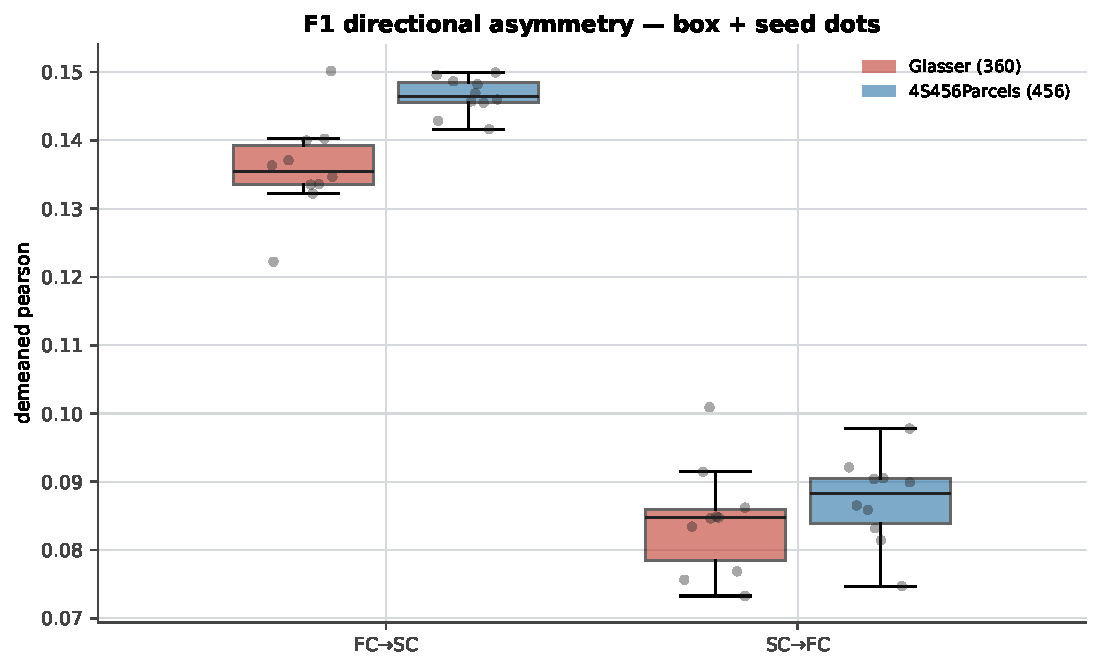
\includegraphics[height=0.82\textheight,width=\linewidth,keepaspectratio]{F1_v_box.pdf}
\end{frame}
\begin{frame}{F1 · Directional asymmetry  (FC$\rightarrow$SC $>$ SC$\rightarrow$FC)}{dumbbell (parcellation gap)}
\centering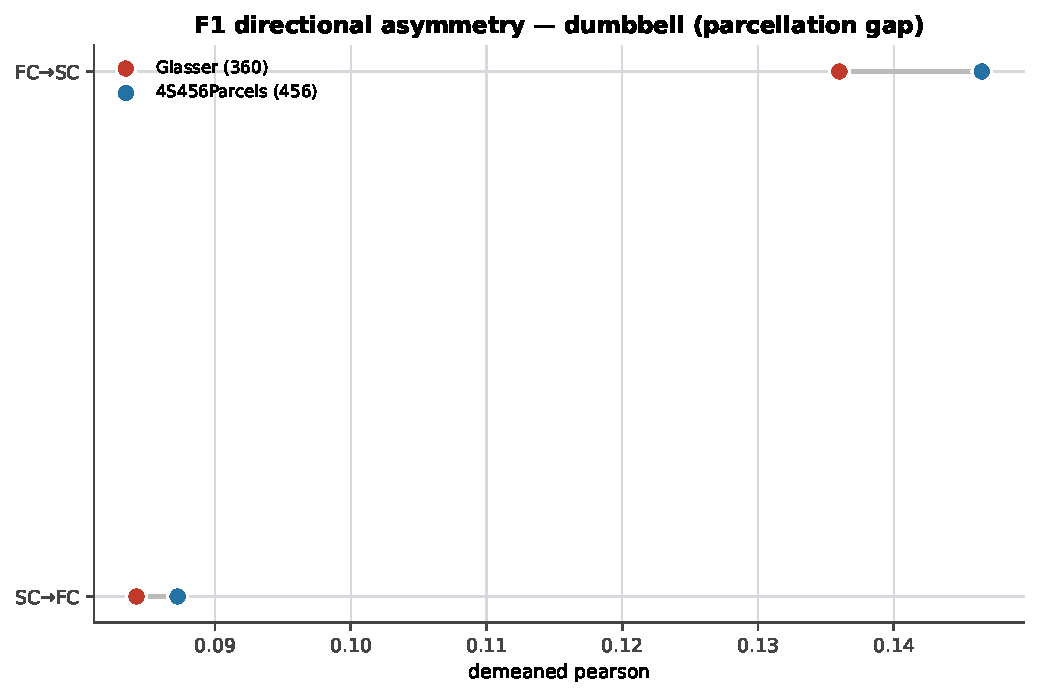
\includegraphics[height=0.82\textheight,width=\linewidth,keepaspectratio]{F1_v_dumbbell.pdf}
\end{frame}
\begin{frame}{F1 · Directional asymmetry  (FC$\rightarrow$SC $>$ SC$\rightarrow$FC)}{grouped bars}
\centering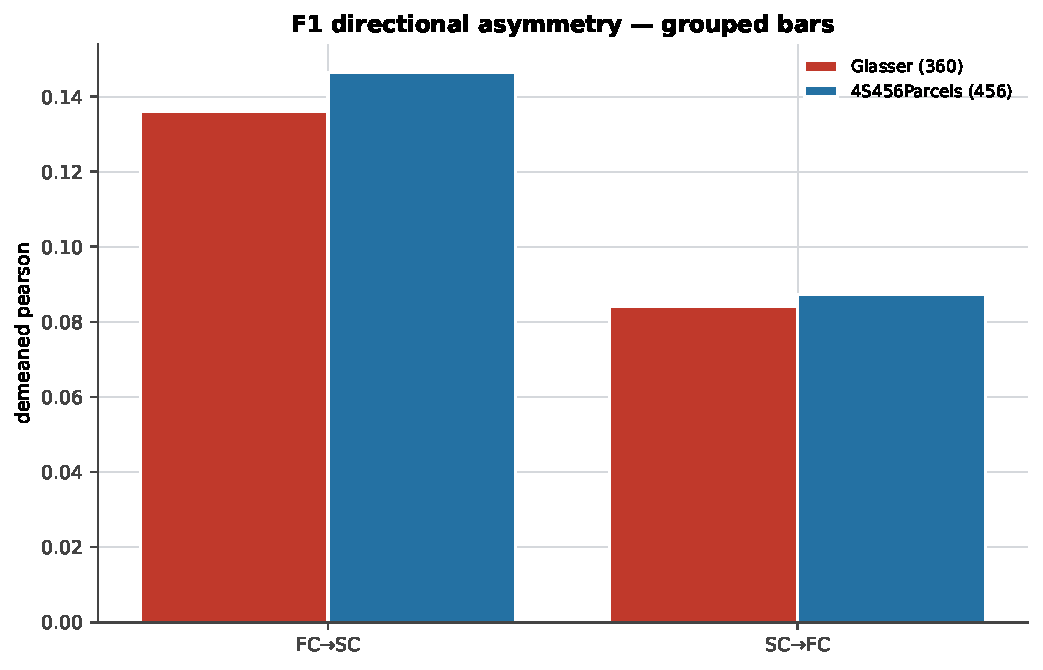
\includegraphics[height=0.82\textheight,width=\linewidth,keepaspectratio]{F1_v_groupedbar.pdf}
\end{frame}
\begin{frame}{F1 · Directional asymmetry  (FC$\rightarrow$SC $>$ SC$\rightarrow$FC)}{horizontal bars}
\centering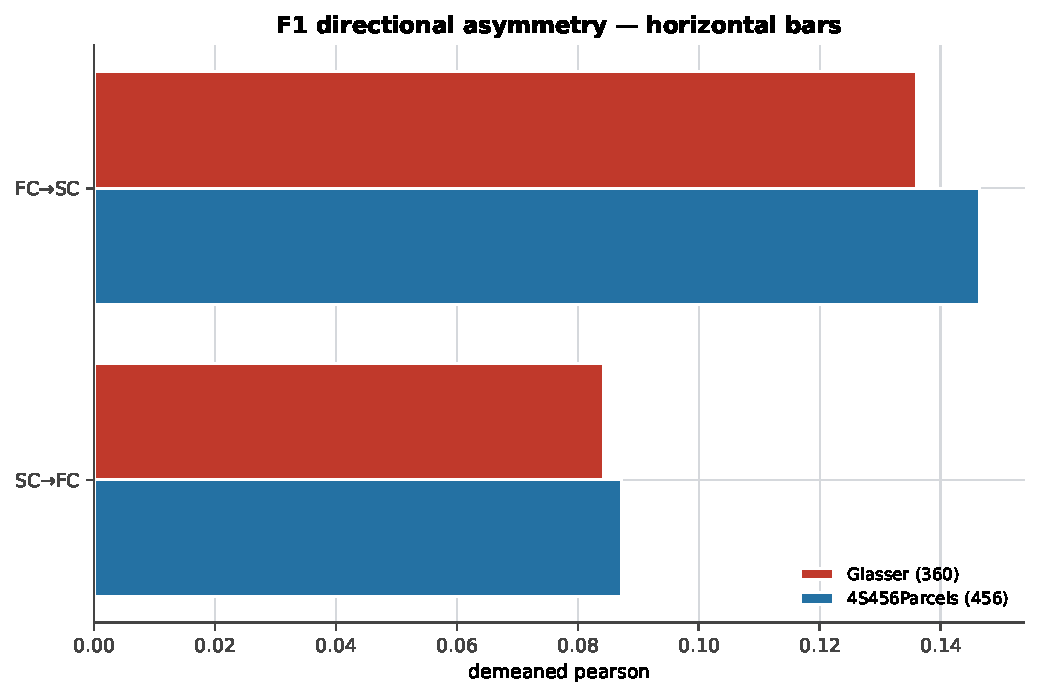
\includegraphics[height=0.82\textheight,width=\linewidth,keepaspectratio]{F1_v_hbar.pdf}
\end{frame}
\begin{frame}{F1 · Directional asymmetry  (FC$\rightarrow$SC $>$ SC$\rightarrow$FC)}{heatmap}
\centering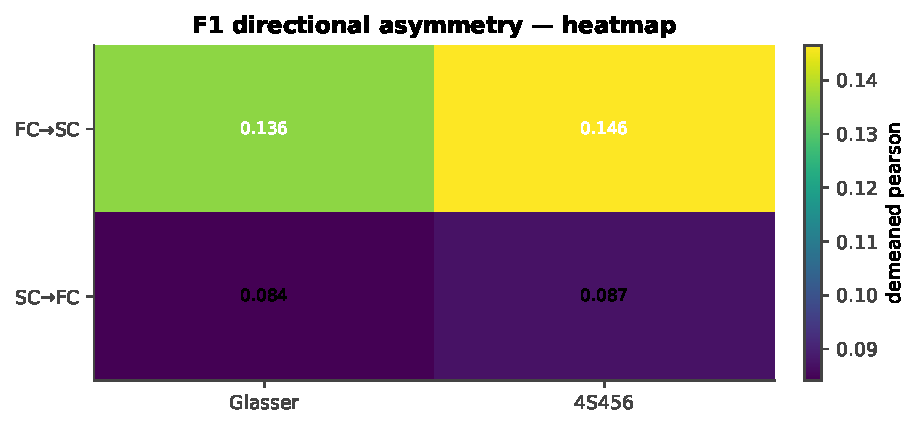
\includegraphics[height=0.82\textheight,width=\linewidth,keepaspectratio]{F1_v_heatmap.pdf}
\end{frame}
\begin{frame}{F1 · Directional asymmetry  (FC$\rightarrow$SC $>$ SC$\rightarrow$FC)}{lollipop}
\centering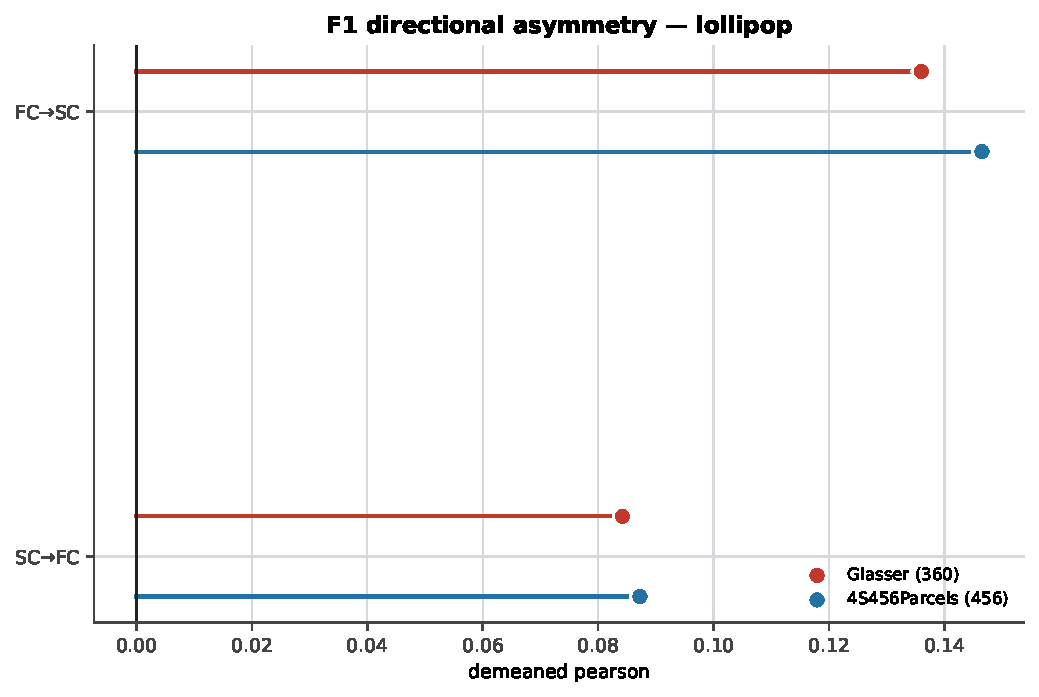
\includegraphics[height=0.82\textheight,width=\linewidth,keepaspectratio]{F1_v_lollipop.pdf}
\end{frame}
\begin{frame}{F1 · Directional asymmetry  (FC$\rightarrow$SC $>$ SC$\rightarrow$FC)}{ratio across estimators}
\centering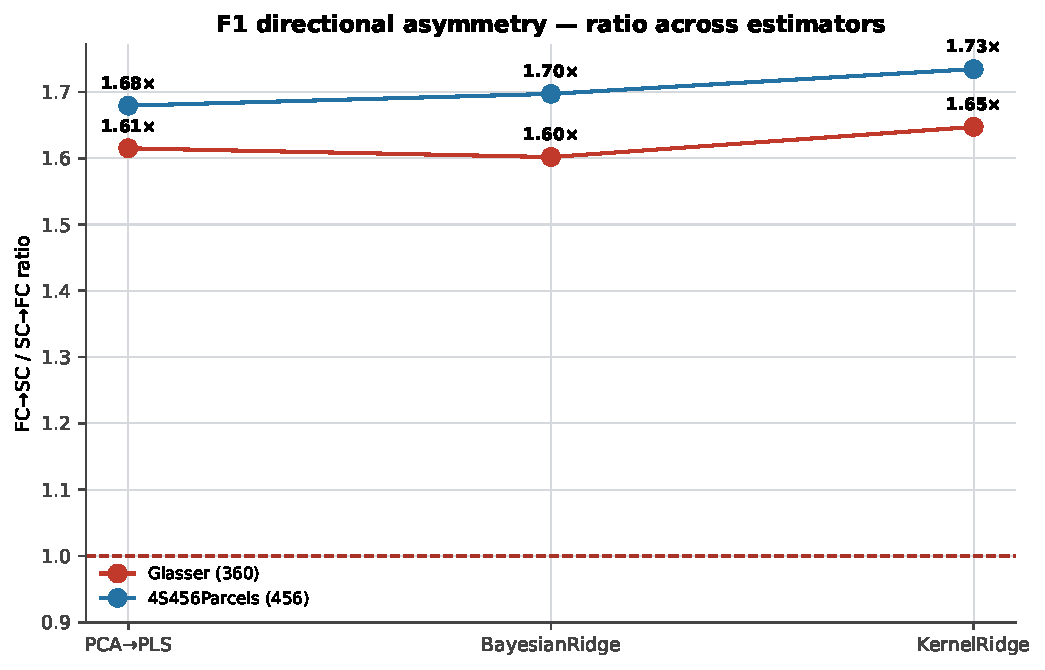
\includegraphics[height=0.82\textheight,width=\linewidth,keepaspectratio]{F1_v_ratioline.pdf}
\end{frame}
\begin{frame}{F1 · Directional asymmetry  (FC$\rightarrow$SC $>$ SC$\rightarrow$FC)}{slope across parcellations}
\centering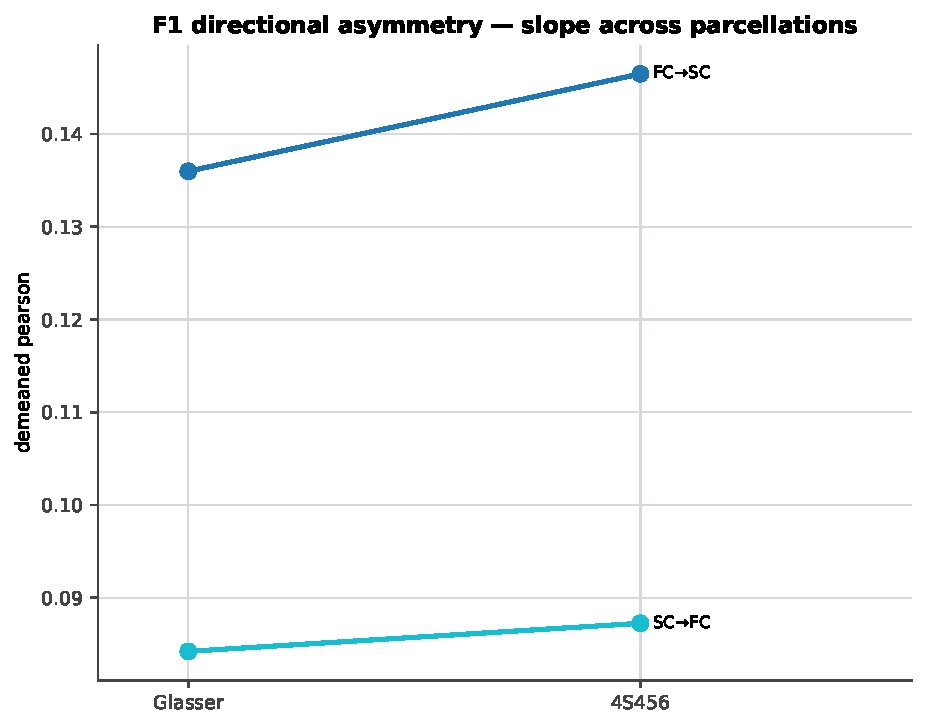
\includegraphics[height=0.82\textheight,width=\linewidth,keepaspectratio]{F1_v_slope.pdf}
\end{frame}
\section{F2}
\begin{frame}\centering\Large\textbf{F2 · Anatomy$\rightarrow$SC / demographics$\rightarrow$FC dissociation}\\[4pt]\normalsize 7 chart variants\end{frame}
\begin{frame}{F2 · Anatomy$\rightarrow$SC / demographics$\rightarrow$FC dissociation}{box + seed dots}
\centering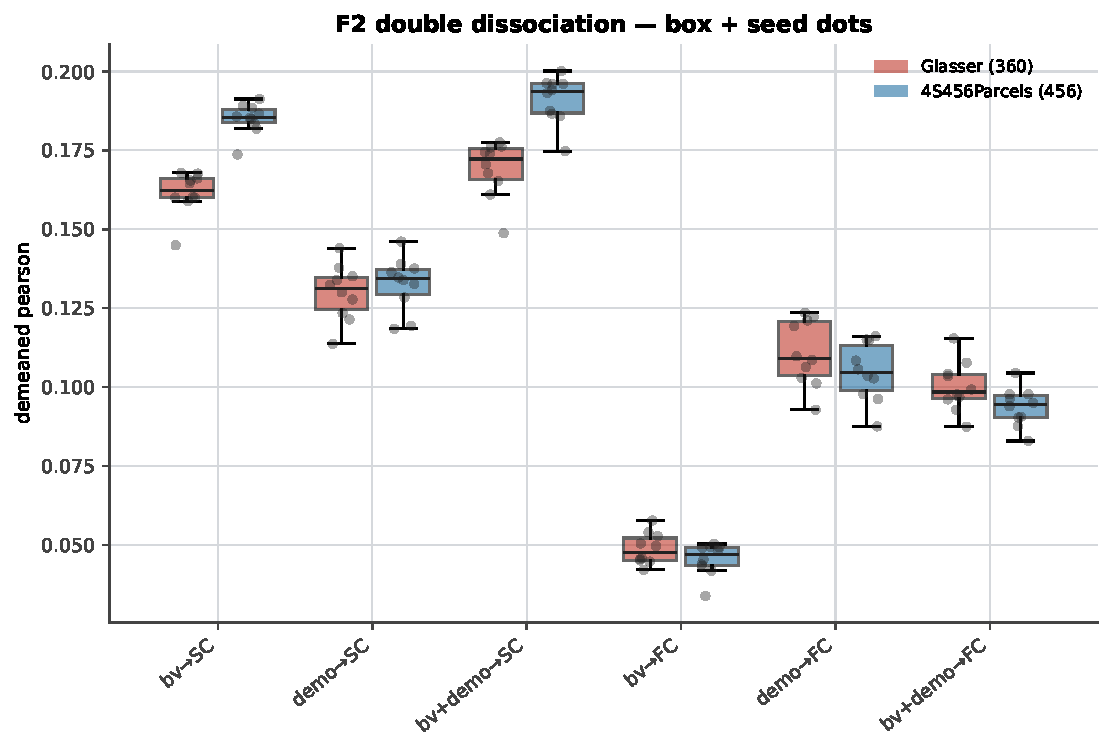
\includegraphics[height=0.82\textheight,width=\linewidth,keepaspectratio]{F2_v_box.pdf}
\end{frame}
\begin{frame}{F2 · Anatomy$\rightarrow$SC / demographics$\rightarrow$FC dissociation}{dumbbell (parcellation gap)}
\centering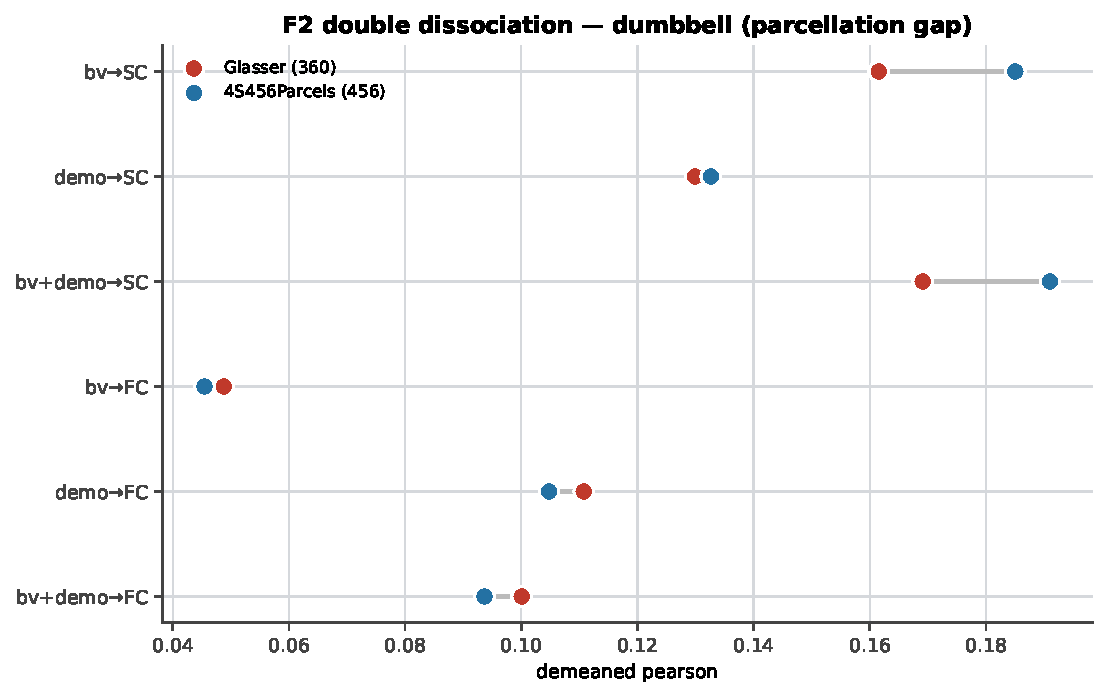
\includegraphics[height=0.82\textheight,width=\linewidth,keepaspectratio]{F2_v_dumbbell.pdf}
\end{frame}
\begin{frame}{F2 · Anatomy$\rightarrow$SC / demographics$\rightarrow$FC dissociation}{grouped bars}
\centering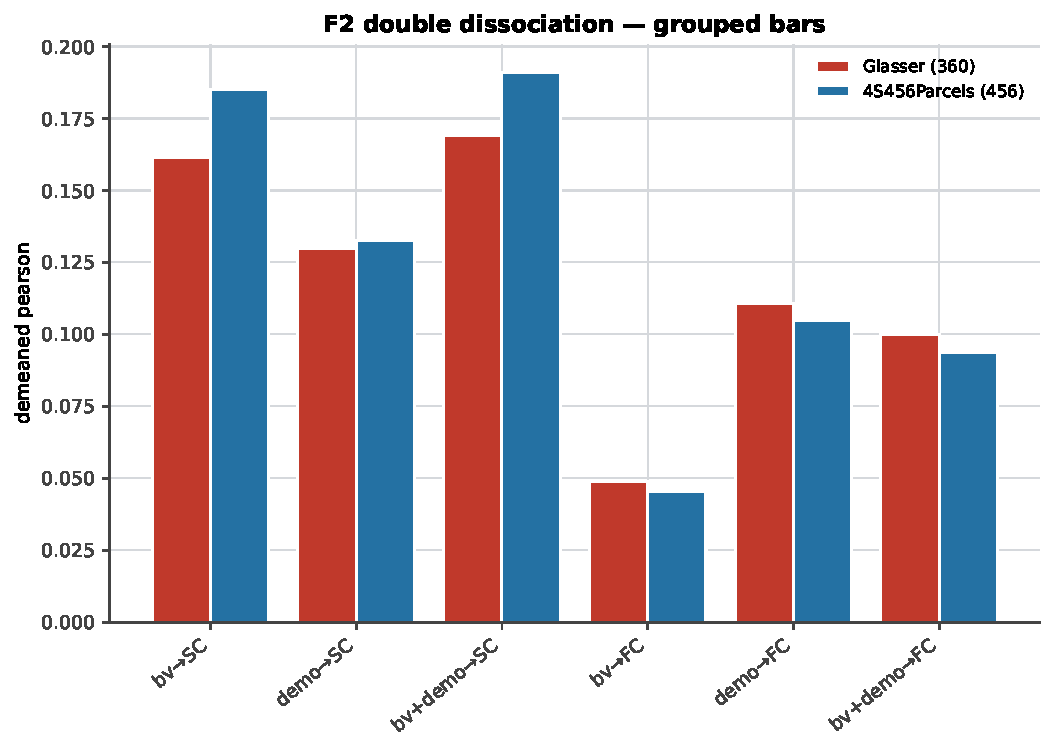
\includegraphics[height=0.82\textheight,width=\linewidth,keepaspectratio]{F2_v_groupedbar.pdf}
\end{frame}
\begin{frame}{F2 · Anatomy$\rightarrow$SC / demographics$\rightarrow$FC dissociation}{horizontal bars}
\centering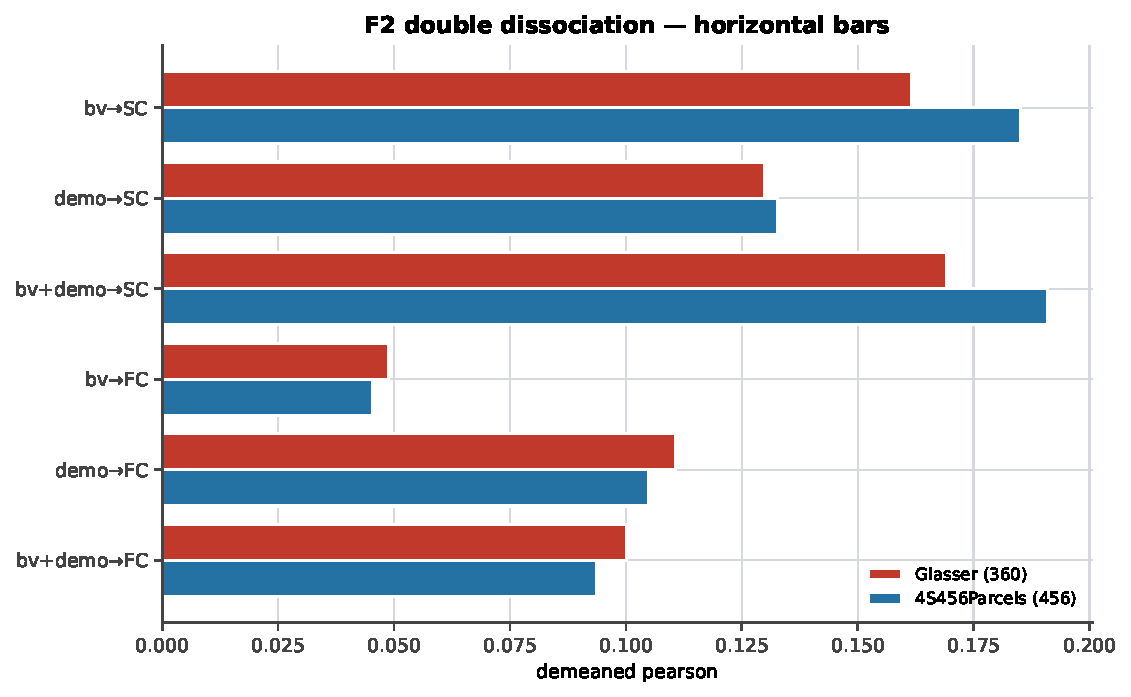
\includegraphics[height=0.82\textheight,width=\linewidth,keepaspectratio]{F2_v_hbar.pdf}
\end{frame}
\begin{frame}{F2 · Anatomy$\rightarrow$SC / demographics$\rightarrow$FC dissociation}{heatmap}
\centering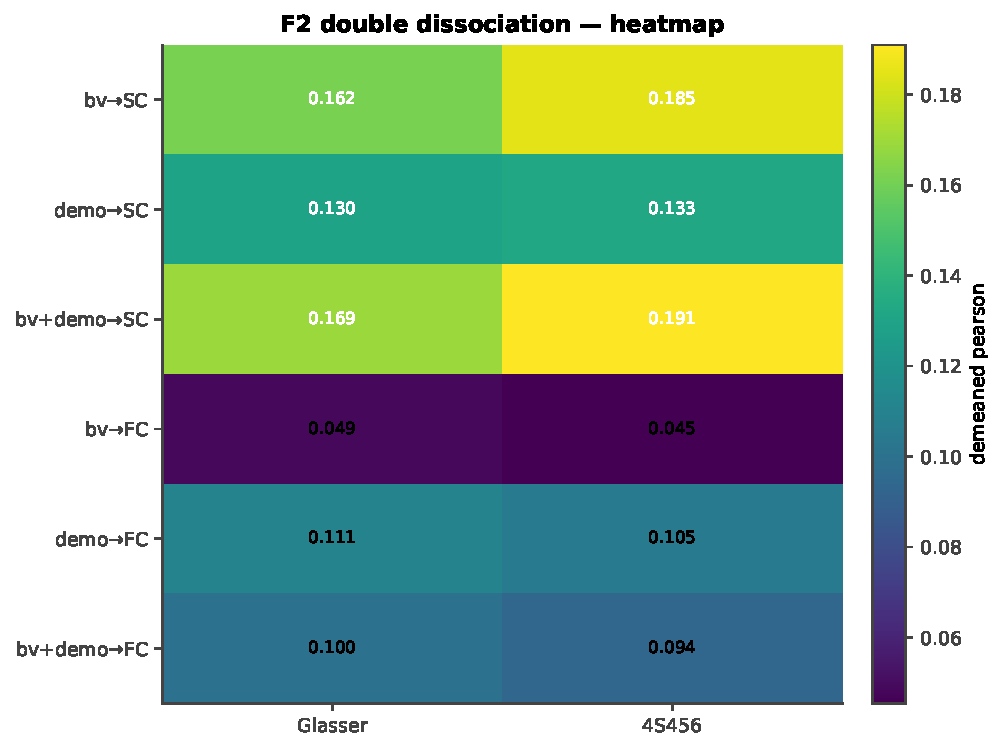
\includegraphics[height=0.82\textheight,width=\linewidth,keepaspectratio]{F2_v_heatmap.pdf}
\end{frame}
\begin{frame}{F2 · Anatomy$\rightarrow$SC / demographics$\rightarrow$FC dissociation}{lollipop}
\centering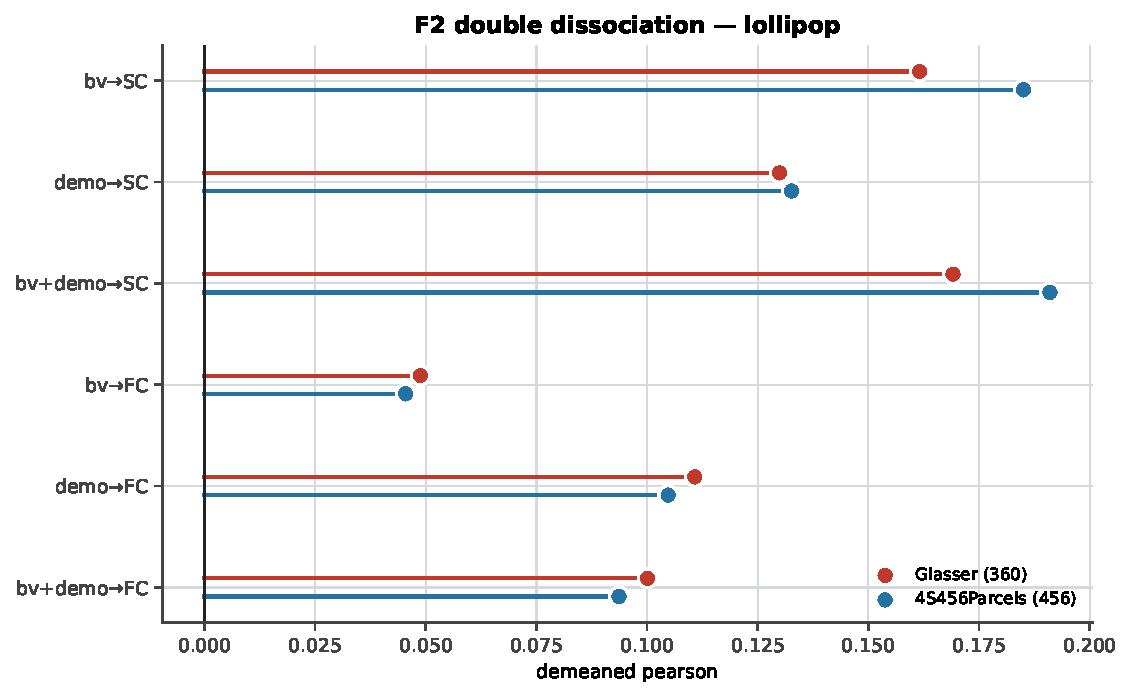
\includegraphics[height=0.82\textheight,width=\linewidth,keepaspectratio]{F2_v_lollipop.pdf}
\end{frame}
\begin{frame}{F2 · Anatomy$\rightarrow$SC / demographics$\rightarrow$FC dissociation}{slope across parcellations}
\centering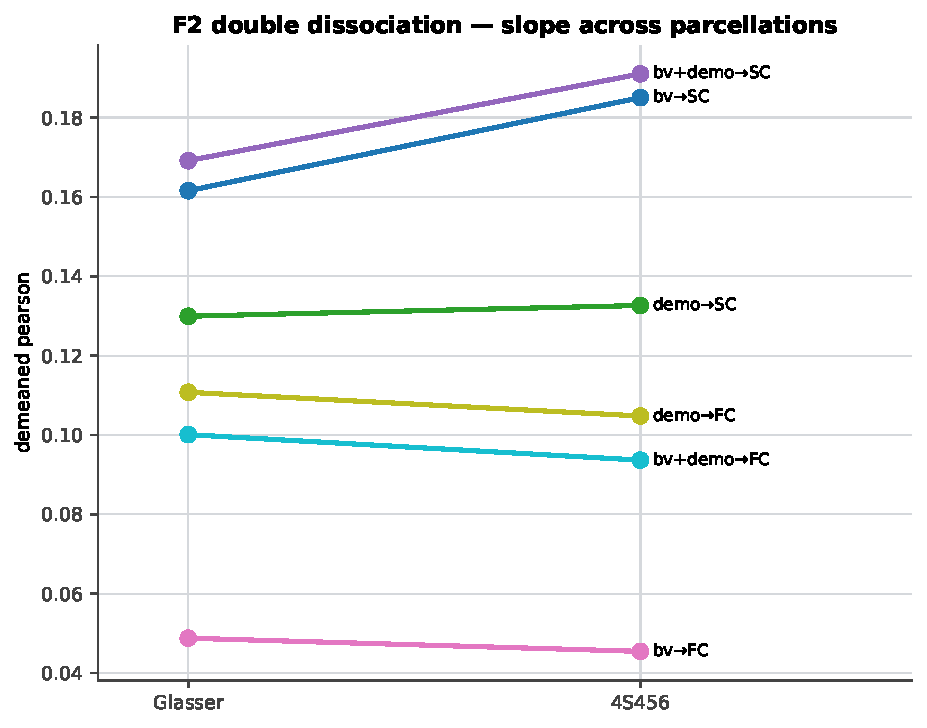
\includegraphics[height=0.82\textheight,width=\linewidth,keepaspectratio]{F2_v_slope.pdf}
\end{frame}
\section{F3}
\begin{frame}\centering\Large\textbf{F3 · Imputed connectomes are measurable}\\[4pt]\normalsize 7 chart variants\end{frame}
\begin{frame}{F3 · Imputed connectomes are measurable}{box + seed dots}
\centering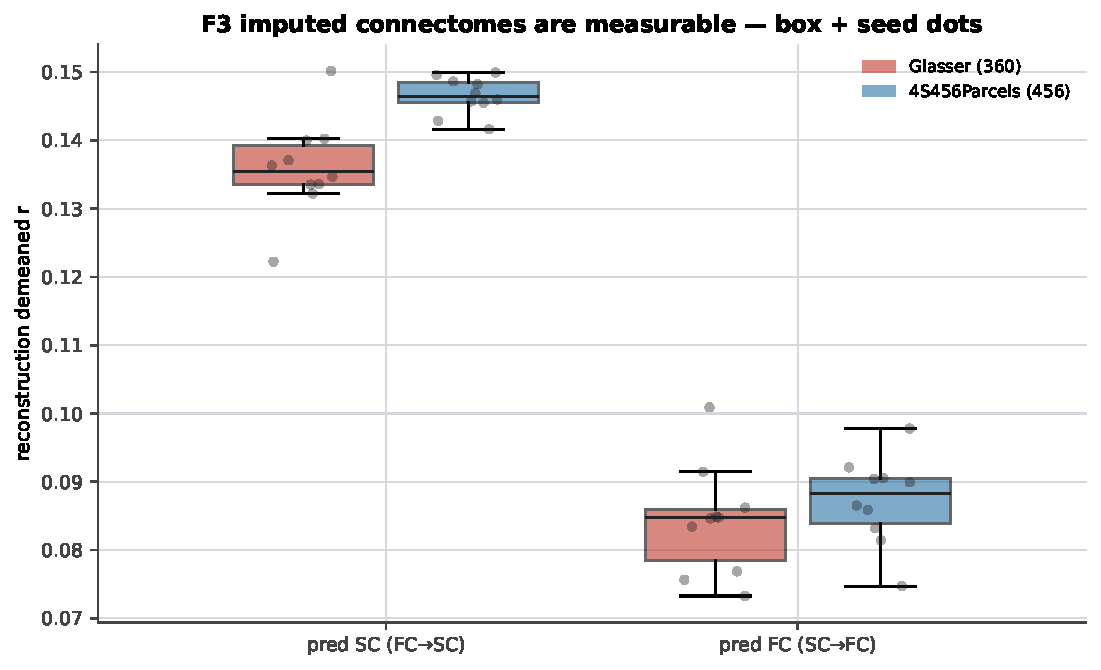
\includegraphics[height=0.82\textheight,width=\linewidth,keepaspectratio]{F3recon_v_box.pdf}
\end{frame}
\begin{frame}{F3 · Imputed connectomes are measurable}{dumbbell (parcellation gap)}
\centering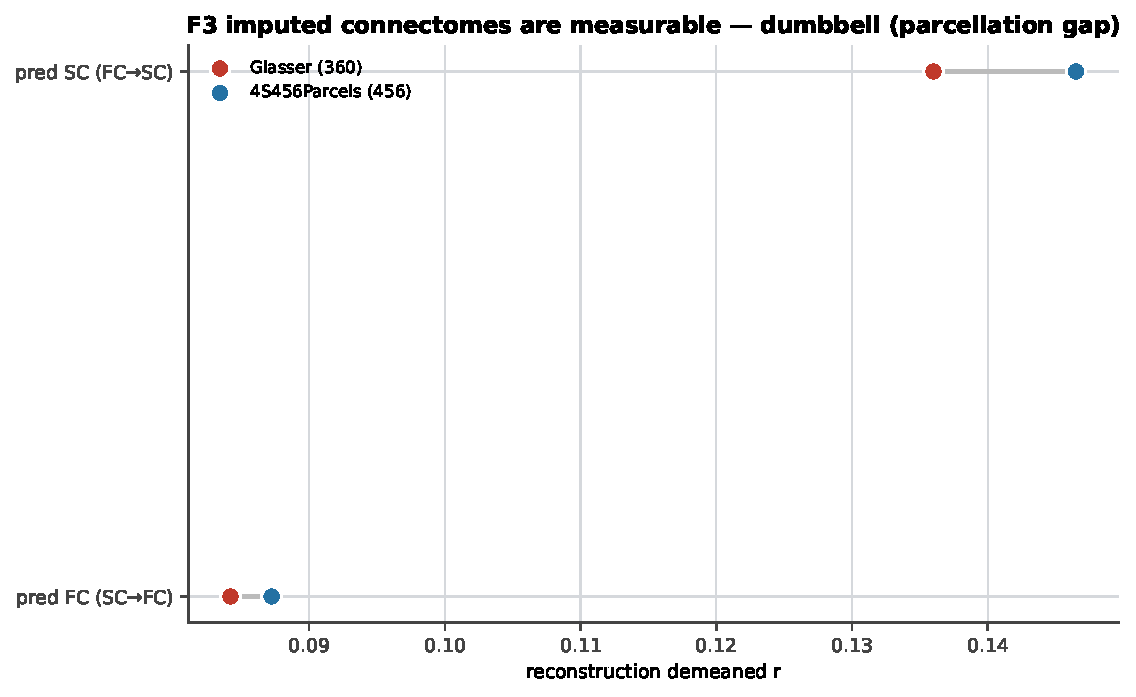
\includegraphics[height=0.82\textheight,width=\linewidth,keepaspectratio]{F3recon_v_dumbbell.pdf}
\end{frame}
\begin{frame}{F3 · Imputed connectomes are measurable}{grouped bars}
\centering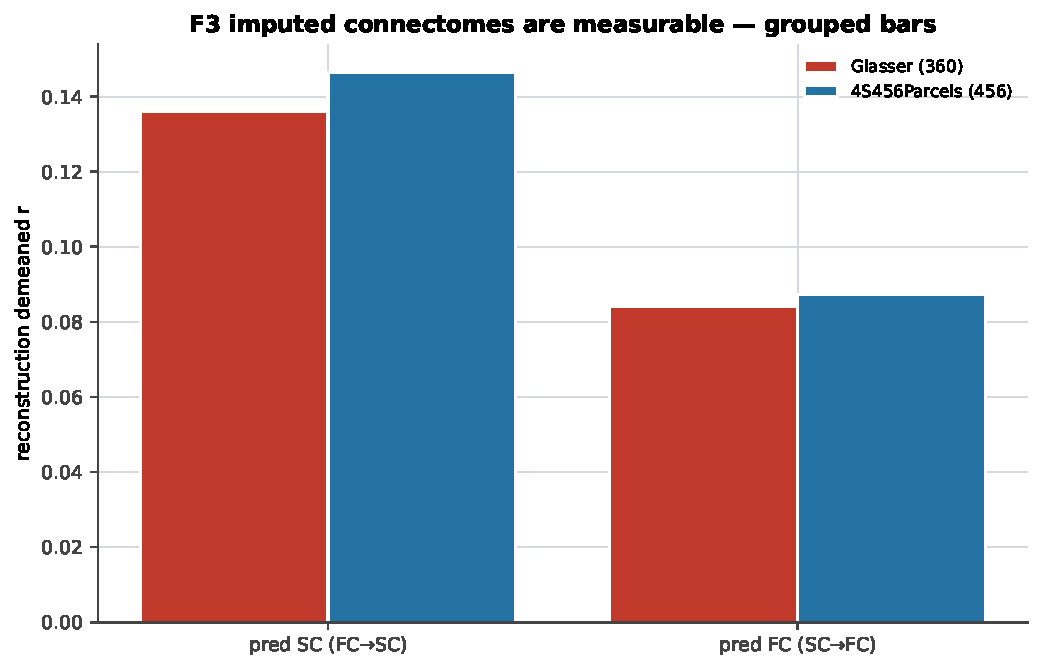
\includegraphics[height=0.82\textheight,width=\linewidth,keepaspectratio]{F3recon_v_groupedbar.pdf}
\end{frame}
\begin{frame}{F3 · Imputed connectomes are measurable}{horizontal bars}
\centering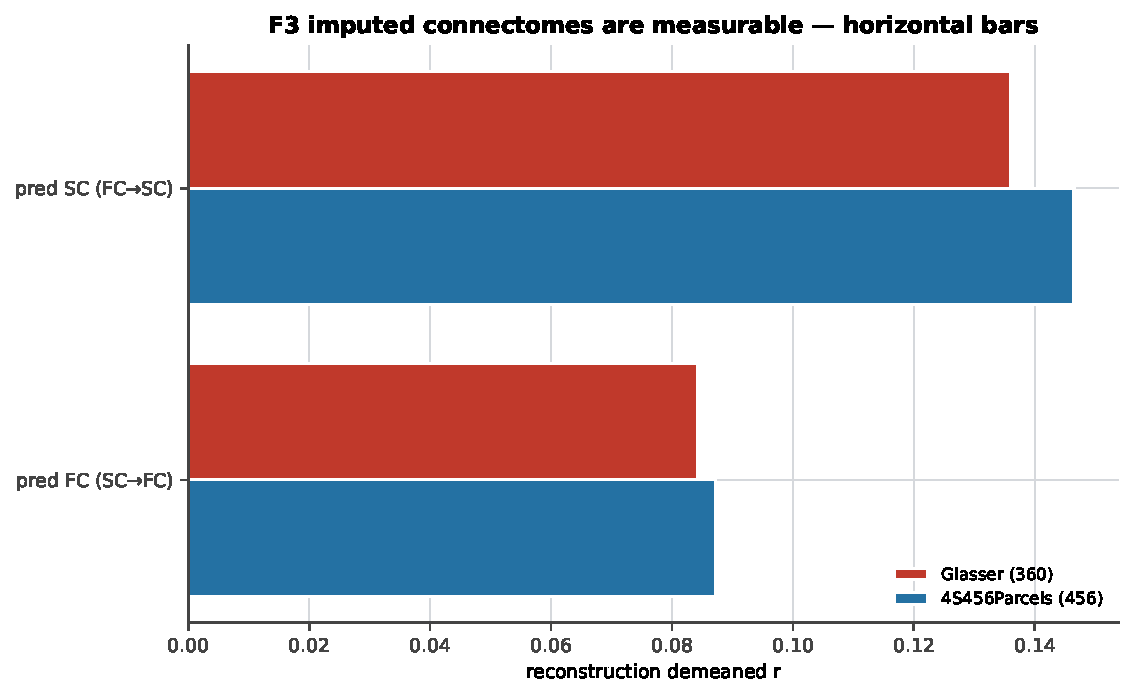
\includegraphics[height=0.82\textheight,width=\linewidth,keepaspectratio]{F3recon_v_hbar.pdf}
\end{frame}
\begin{frame}{F3 · Imputed connectomes are measurable}{heatmap}
\centering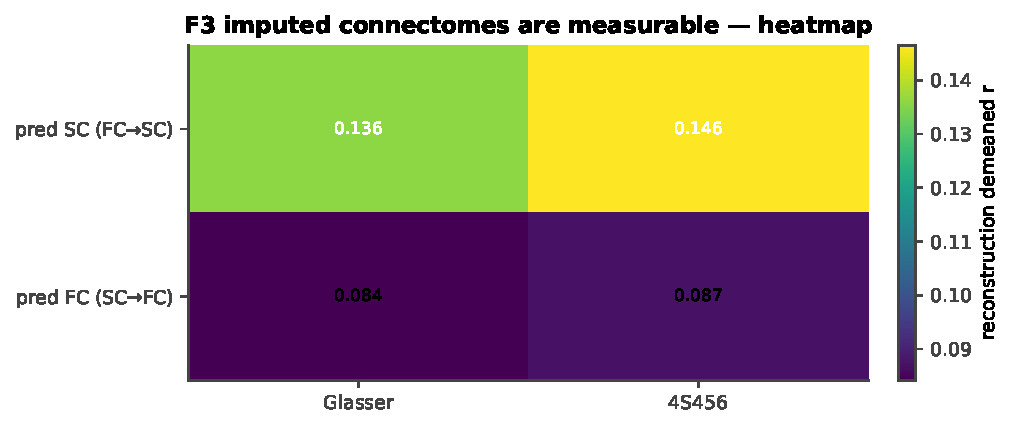
\includegraphics[height=0.82\textheight,width=\linewidth,keepaspectratio]{F3recon_v_heatmap.pdf}
\end{frame}
\begin{frame}{F3 · Imputed connectomes are measurable}{lollipop}
\centering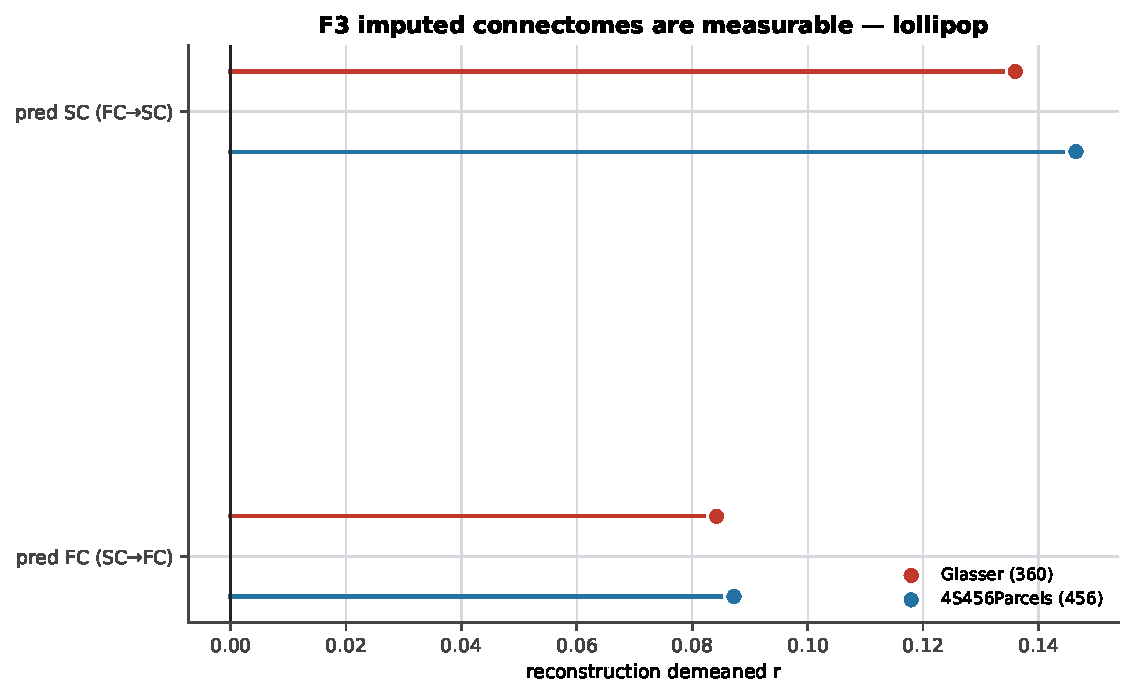
\includegraphics[height=0.82\textheight,width=\linewidth,keepaspectratio]{F3recon_v_lollipop.pdf}
\end{frame}
\begin{frame}{F3 · Imputed connectomes are measurable}{slope across parcellations}
\centering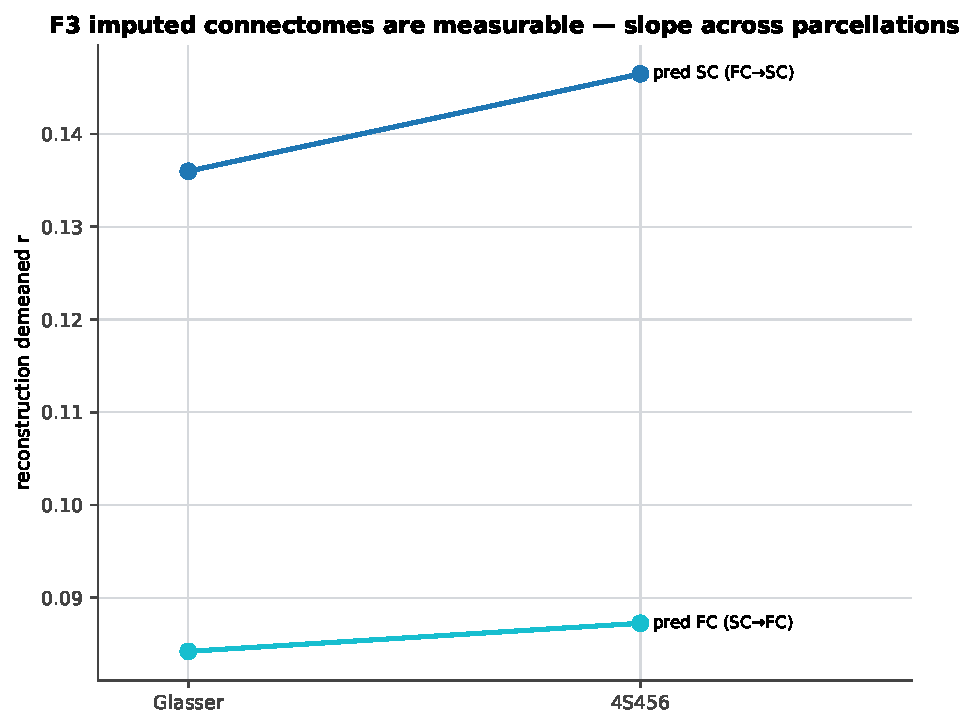
\includegraphics[height=0.82\textheight,width=\linewidth,keepaspectratio]{F3recon_v_slope.pdf}
\end{frame}
\section{F3}
\begin{frame}\centering\Large\textbf{F3 · …but their utility is asymmetric}\\[4pt]\normalsize 7 chart variants\end{frame}
\begin{frame}{F3 · …but their utility is asymmetric}{box + seed dots}
\centering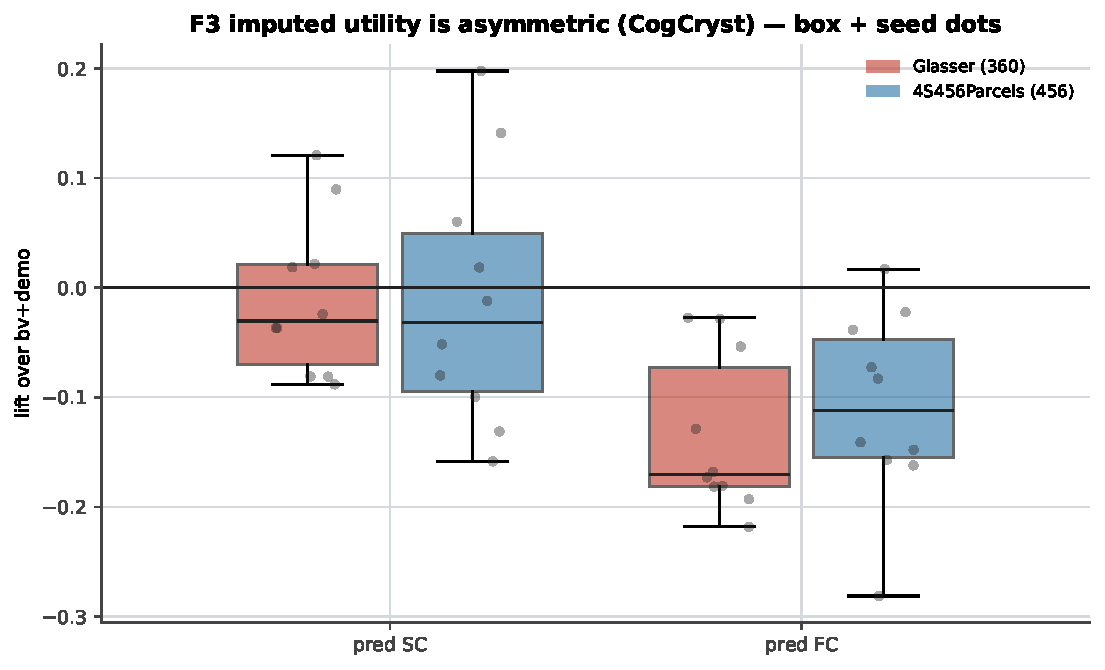
\includegraphics[height=0.82\textheight,width=\linewidth,keepaspectratio]{F3util_v_box.pdf}
\end{frame}
\begin{frame}{F3 · …but their utility is asymmetric}{dumbbell (parcellation gap)}
\centering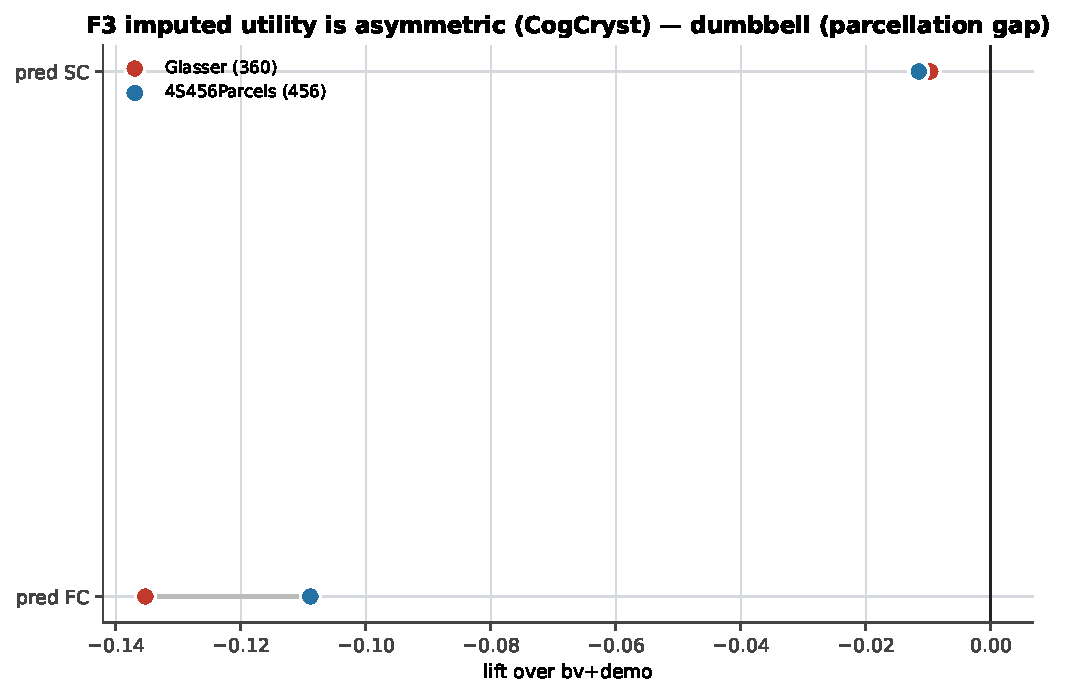
\includegraphics[height=0.82\textheight,width=\linewidth,keepaspectratio]{F3util_v_dumbbell.pdf}
\end{frame}
\begin{frame}{F3 · …but their utility is asymmetric}{grouped bars}
\centering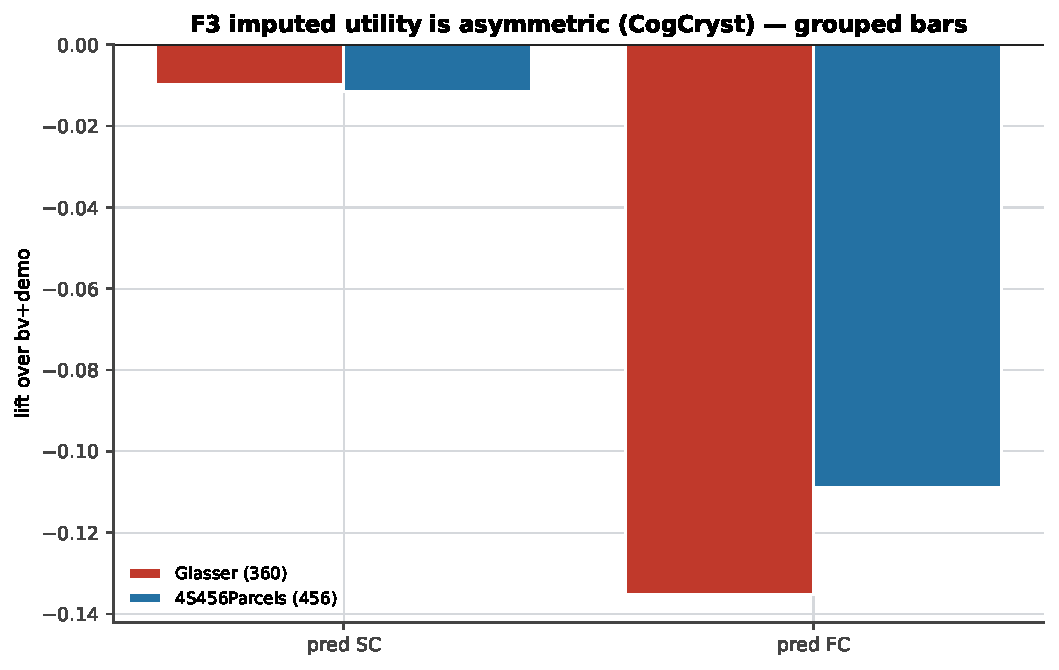
\includegraphics[height=0.82\textheight,width=\linewidth,keepaspectratio]{F3util_v_groupedbar.pdf}
\end{frame}
\begin{frame}{F3 · …but their utility is asymmetric}{horizontal bars}
\centering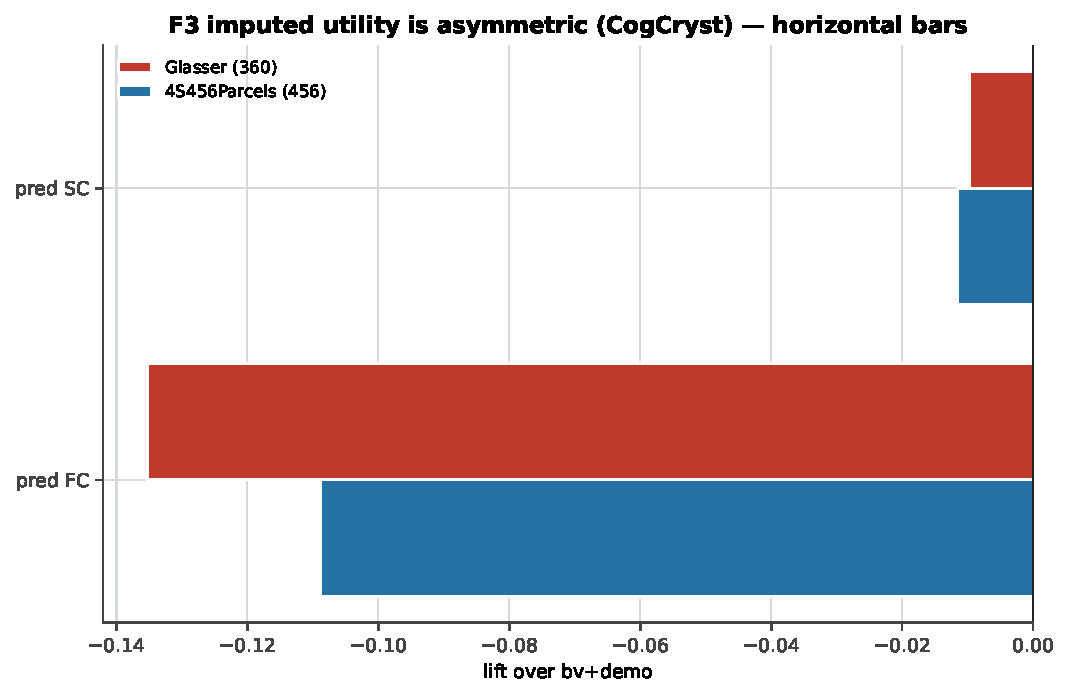
\includegraphics[height=0.82\textheight,width=\linewidth,keepaspectratio]{F3util_v_hbar.pdf}
\end{frame}
\begin{frame}{F3 · …but their utility is asymmetric}{heatmap}
\centering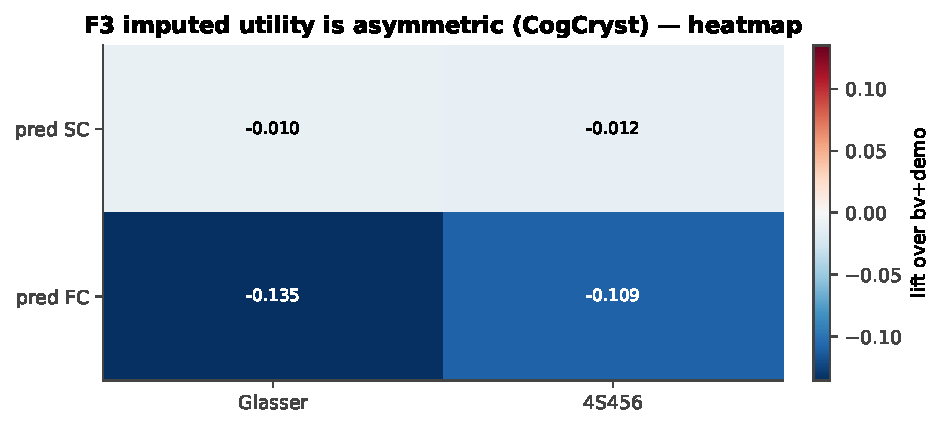
\includegraphics[height=0.82\textheight,width=\linewidth,keepaspectratio]{F3util_v_heatmap.pdf}
\end{frame}
\begin{frame}{F3 · …but their utility is asymmetric}{lollipop}
\centering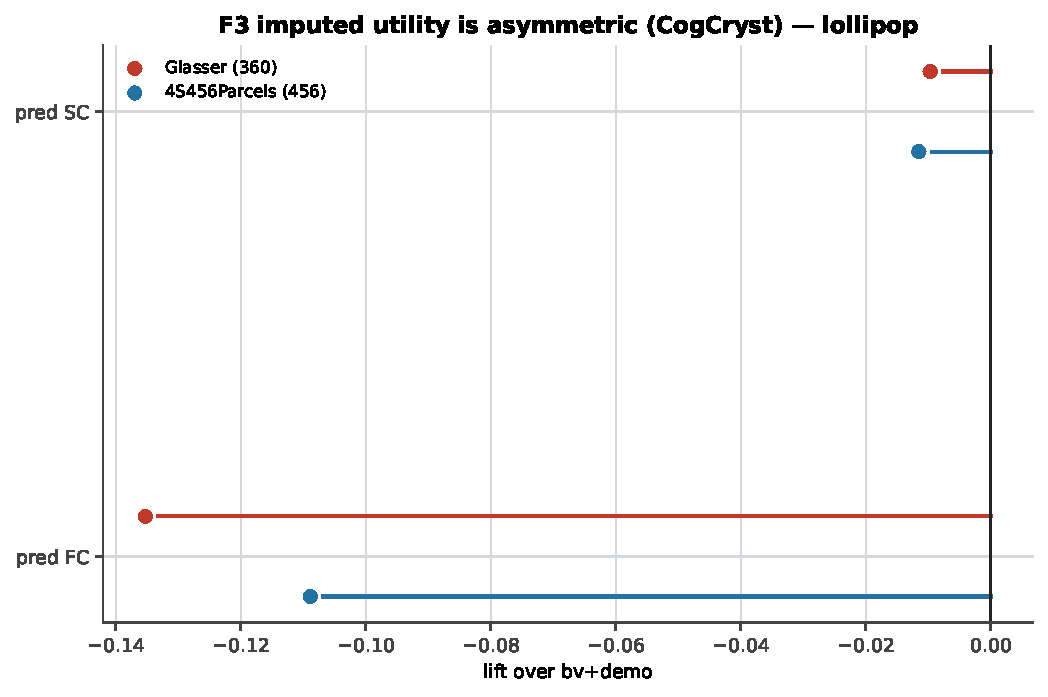
\includegraphics[height=0.82\textheight,width=\linewidth,keepaspectratio]{F3util_v_lollipop.pdf}
\end{frame}
\begin{frame}{F3 · …but their utility is asymmetric}{slope across parcellations}
\centering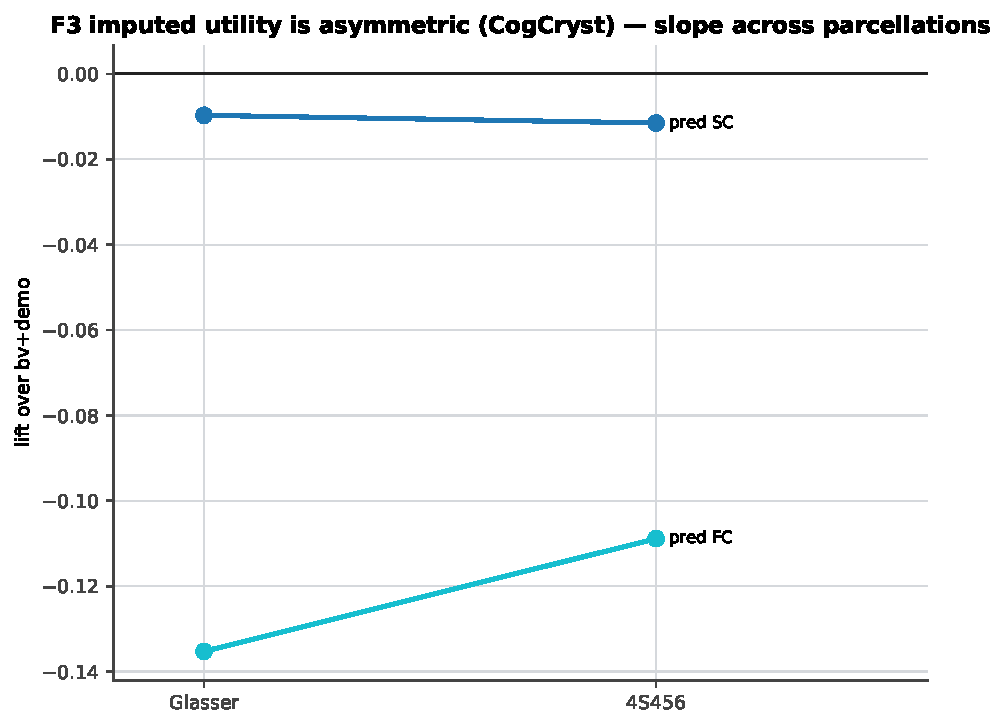
\includegraphics[height=0.82\textheight,width=\linewidth,keepaspectratio]{F3util_v_slope.pdf}
\end{frame}
\section{F4}
\begin{frame}\centering\Large\textbf{F4 · Observed FC: crystallized-cognition signal (narrow, FDR-surviving)}\\[4pt]\normalsize 7 chart variants\end{frame}
\begin{frame}{F4 · Observed FC: crystallized-cognition signal (narrow, FDR-surviving)}{box + seed dots}
\centering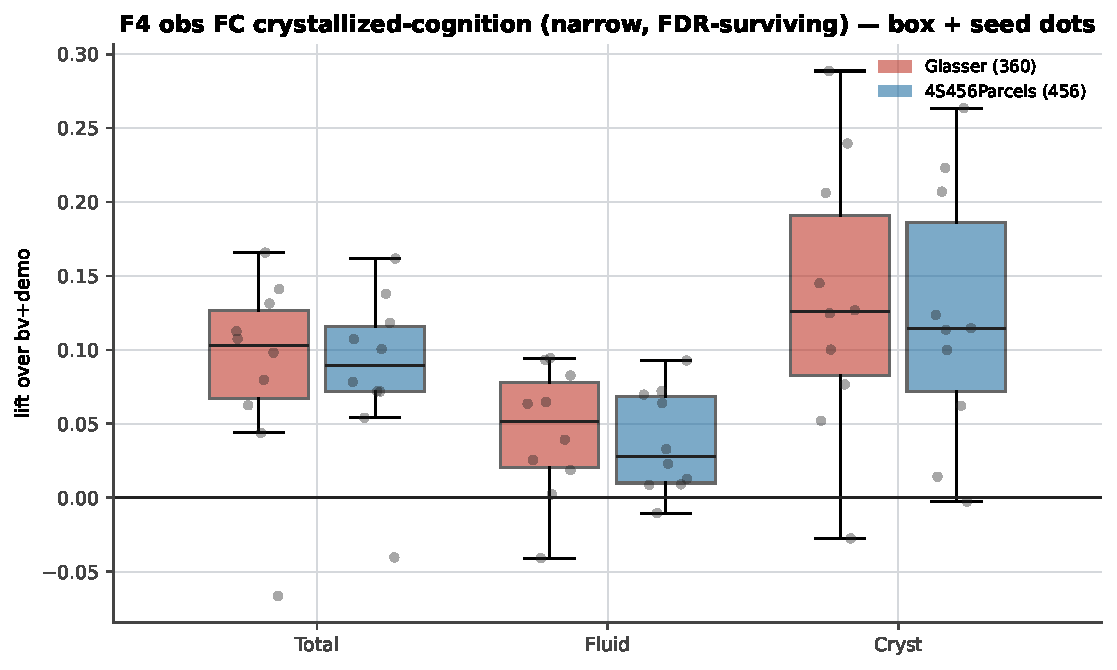
\includegraphics[height=0.82\textheight,width=\linewidth,keepaspectratio]{F4_v_box.pdf}
\end{frame}
\begin{frame}{F4 · Observed FC: crystallized-cognition signal (narrow, FDR-surviving)}{dumbbell (parcellation gap)}
\centering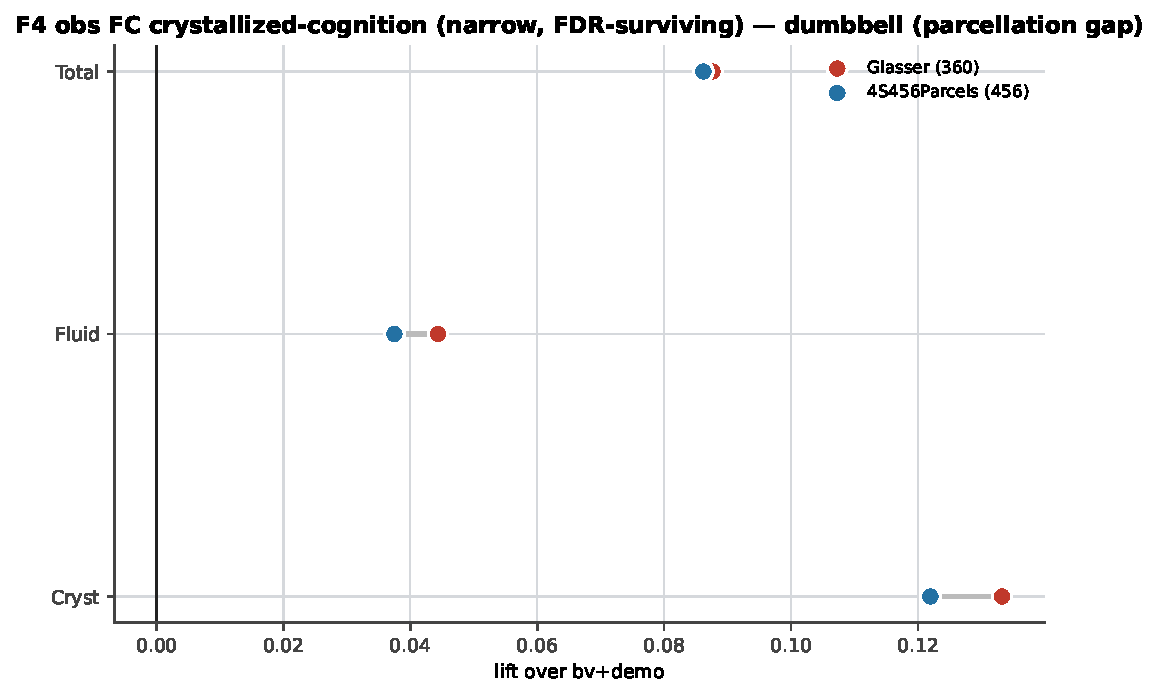
\includegraphics[height=0.82\textheight,width=\linewidth,keepaspectratio]{F4_v_dumbbell.pdf}
\end{frame}
\begin{frame}{F4 · Observed FC: crystallized-cognition signal (narrow, FDR-surviving)}{grouped bars}
\centering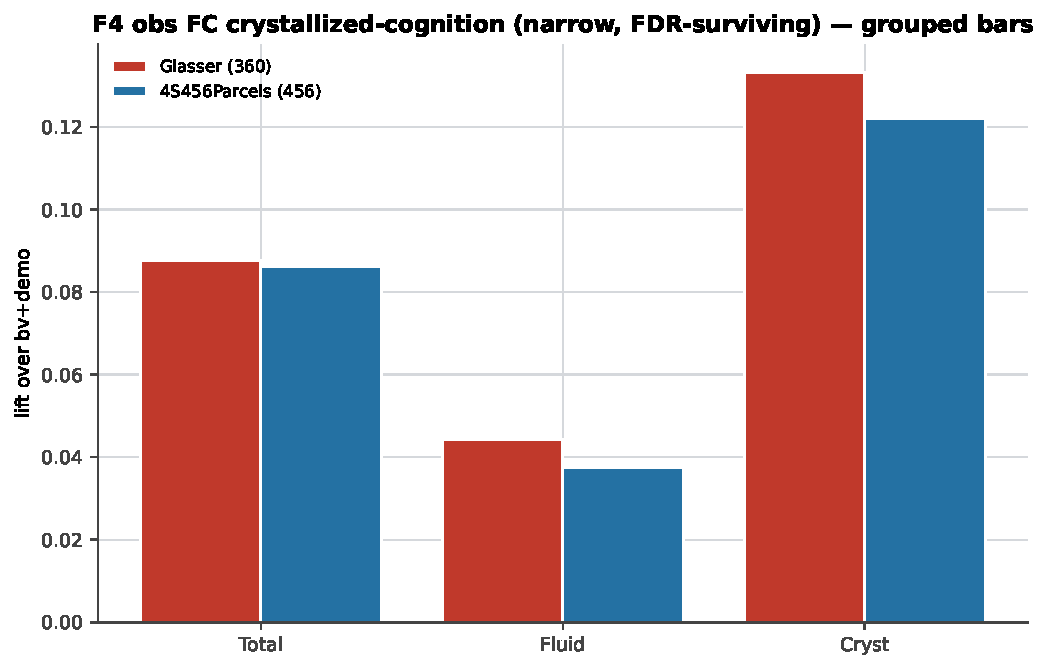
\includegraphics[height=0.82\textheight,width=\linewidth,keepaspectratio]{F4_v_groupedbar.pdf}
\end{frame}
\begin{frame}{F4 · Observed FC: crystallized-cognition signal (narrow, FDR-surviving)}{horizontal bars}
\centering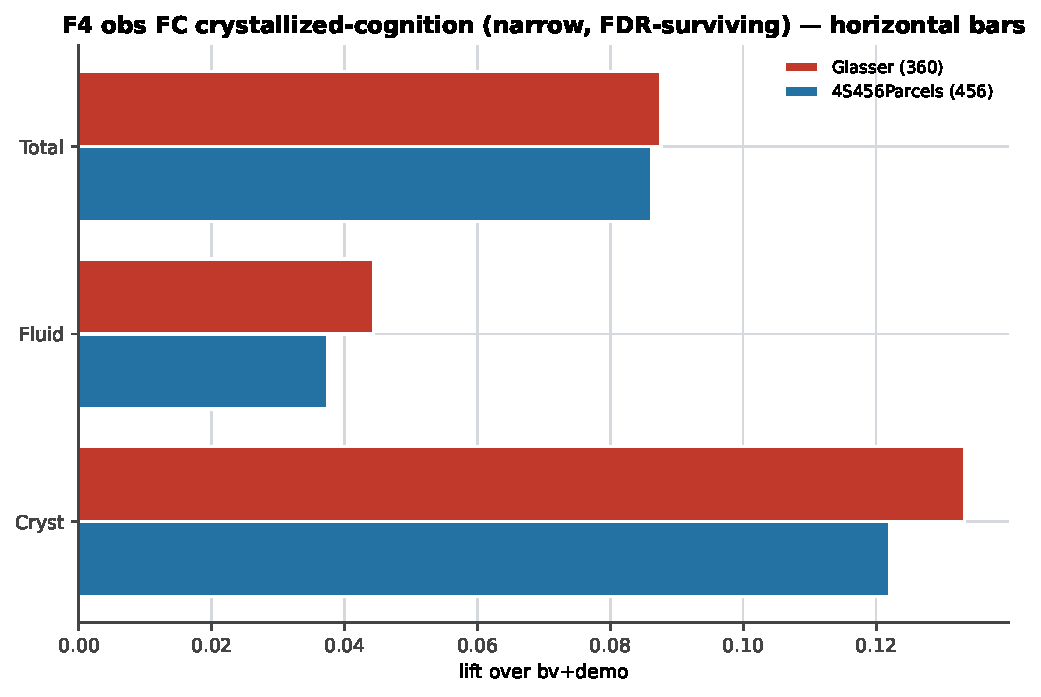
\includegraphics[height=0.82\textheight,width=\linewidth,keepaspectratio]{F4_v_hbar.pdf}
\end{frame}
\begin{frame}{F4 · Observed FC: crystallized-cognition signal (narrow, FDR-surviving)}{heatmap}
\centering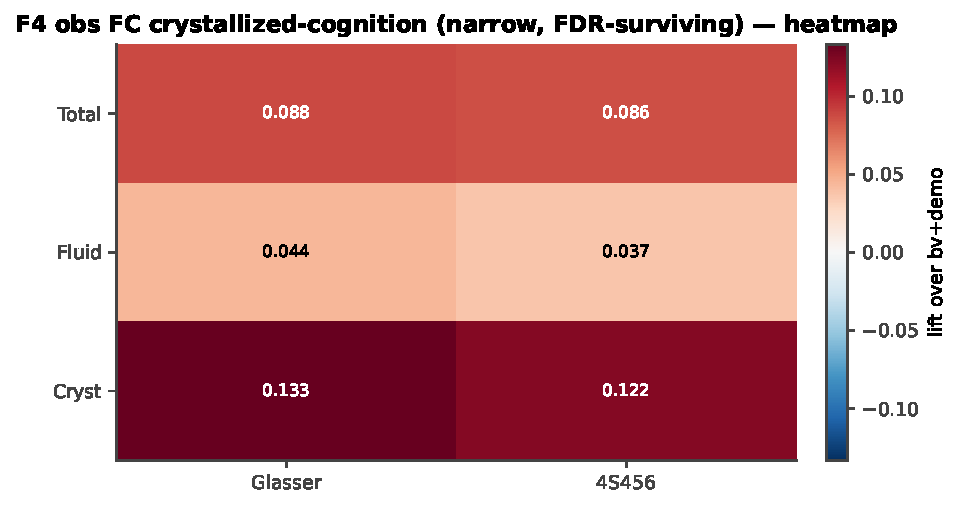
\includegraphics[height=0.82\textheight,width=\linewidth,keepaspectratio]{F4_v_heatmap.pdf}
\end{frame}
\begin{frame}{F4 · Observed FC: crystallized-cognition signal (narrow, FDR-surviving)}{lollipop}
\centering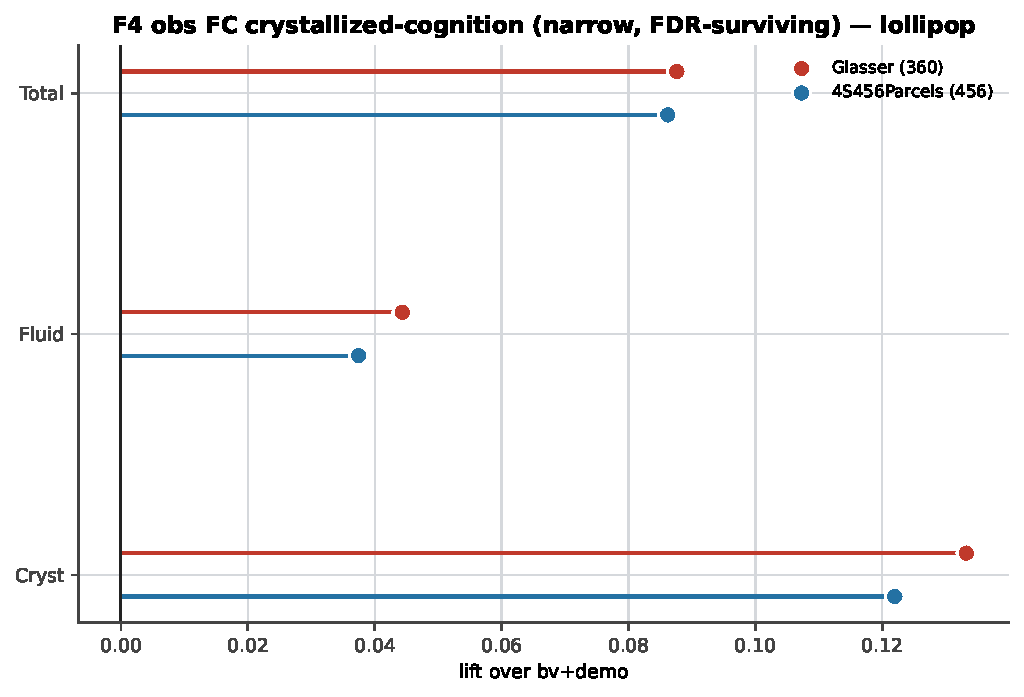
\includegraphics[height=0.82\textheight,width=\linewidth,keepaspectratio]{F4_v_lollipop.pdf}
\end{frame}
\begin{frame}{F4 · Observed FC: crystallized-cognition signal (narrow, FDR-surviving)}{slope across parcellations}
\centering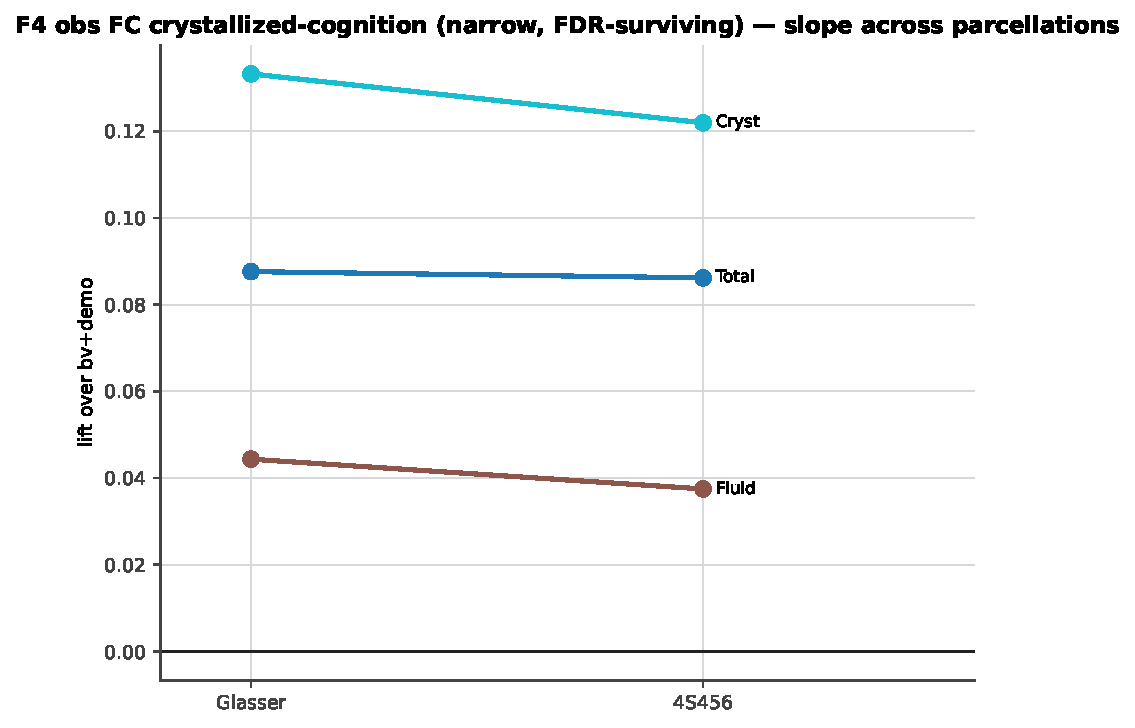
\includegraphics[height=0.82\textheight,width=\linewidth,keepaspectratio]{F4_v_slope.pdf}
\end{frame}
\section{F5}
\begin{frame}\centering\Large\textbf{F5 · SC / imputation utility wall}\\[4pt]\normalsize 7 chart variants\end{frame}
\begin{frame}{F5 · SC / imputation utility wall}{box + seed dots}
\centering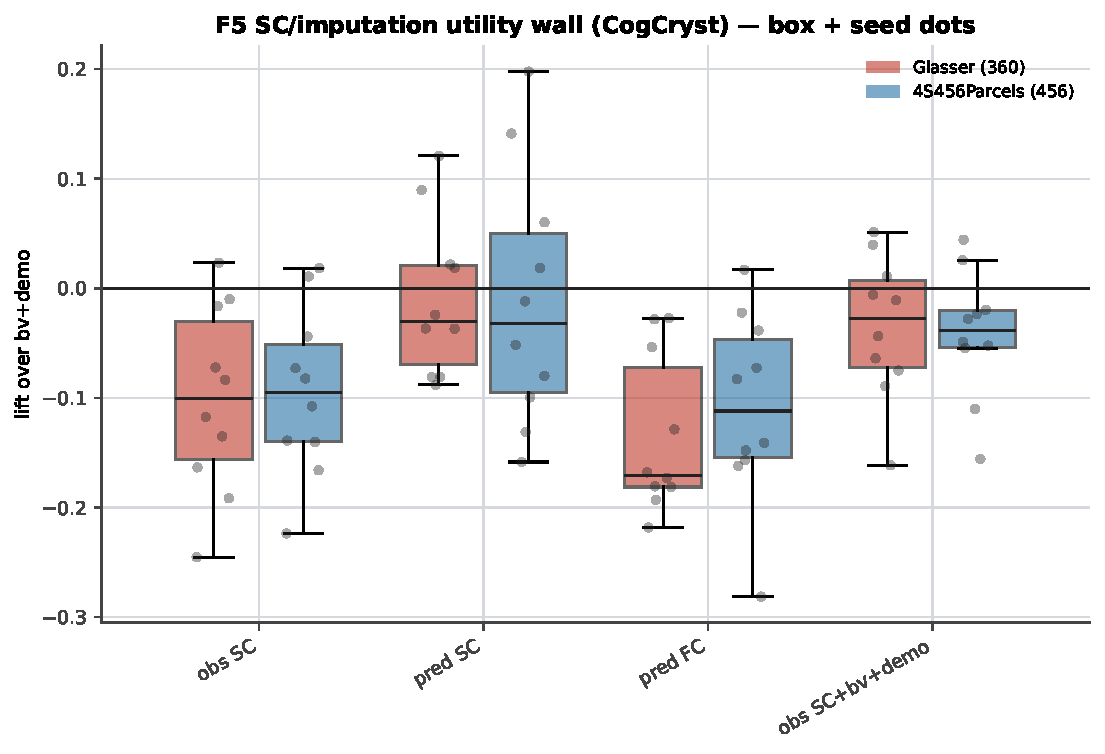
\includegraphics[height=0.82\textheight,width=\linewidth,keepaspectratio]{F5_v_box.pdf}
\end{frame}
\begin{frame}{F5 · SC / imputation utility wall}{dumbbell (parcellation gap)}
\centering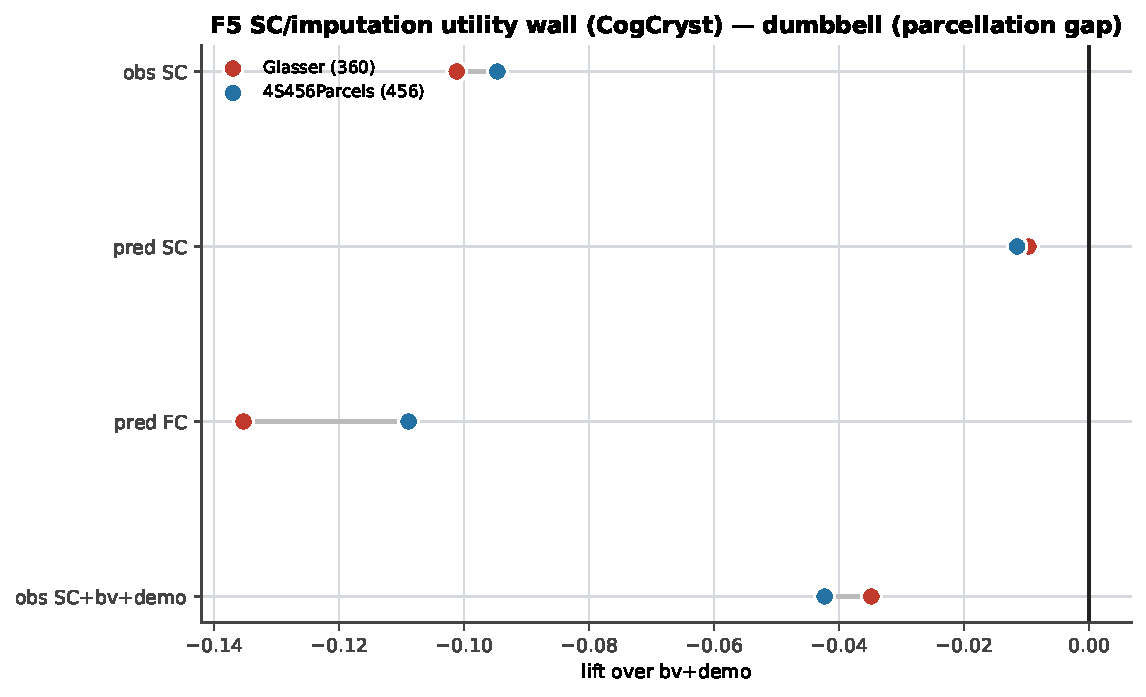
\includegraphics[height=0.82\textheight,width=\linewidth,keepaspectratio]{F5_v_dumbbell.pdf}
\end{frame}
\begin{frame}{F5 · SC / imputation utility wall}{grouped bars}
\centering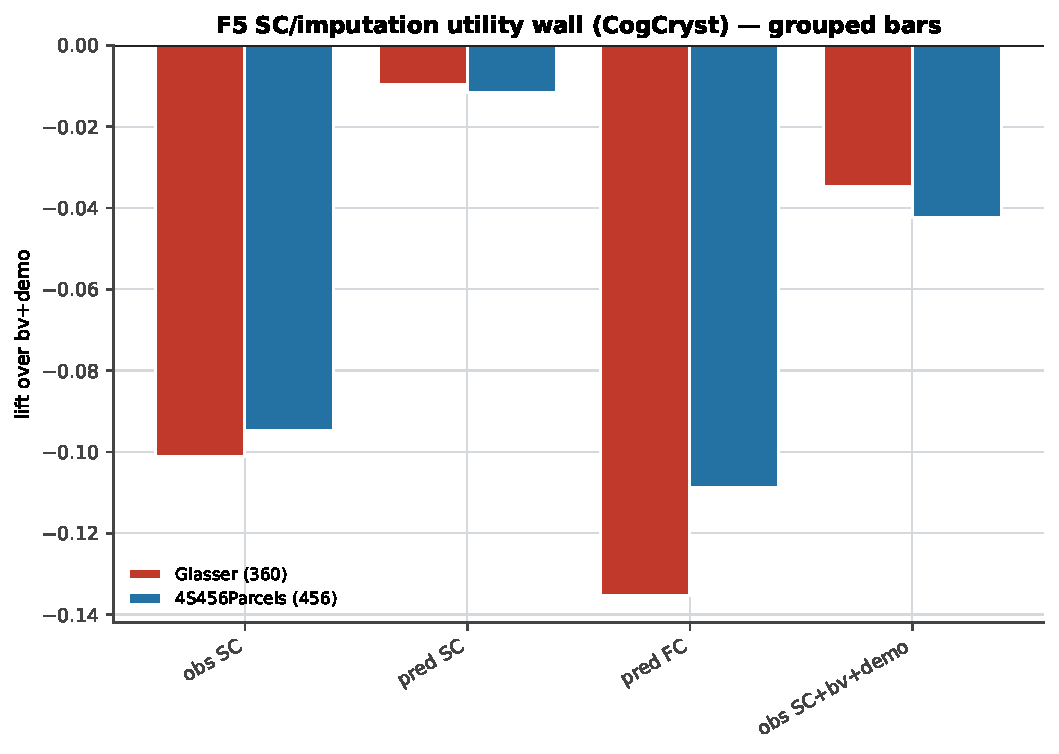
\includegraphics[height=0.82\textheight,width=\linewidth,keepaspectratio]{F5_v_groupedbar.pdf}
\end{frame}
\begin{frame}{F5 · SC / imputation utility wall}{horizontal bars}
\centering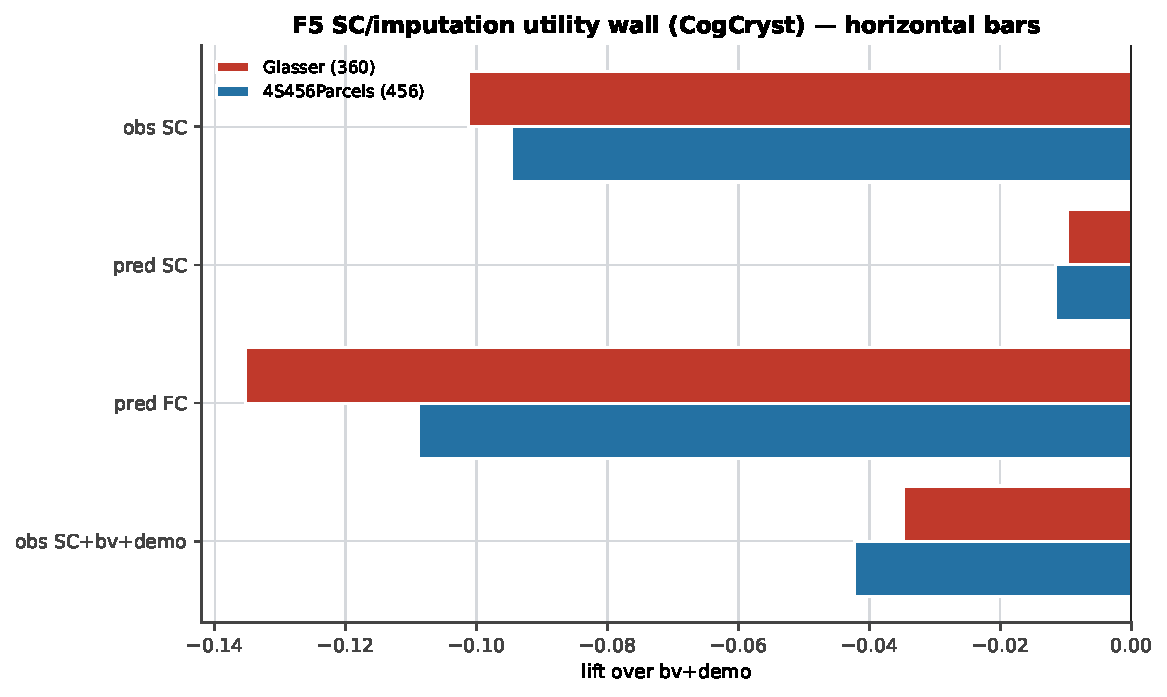
\includegraphics[height=0.82\textheight,width=\linewidth,keepaspectratio]{F5_v_hbar.pdf}
\end{frame}
\begin{frame}{F5 · SC / imputation utility wall}{heatmap}
\centering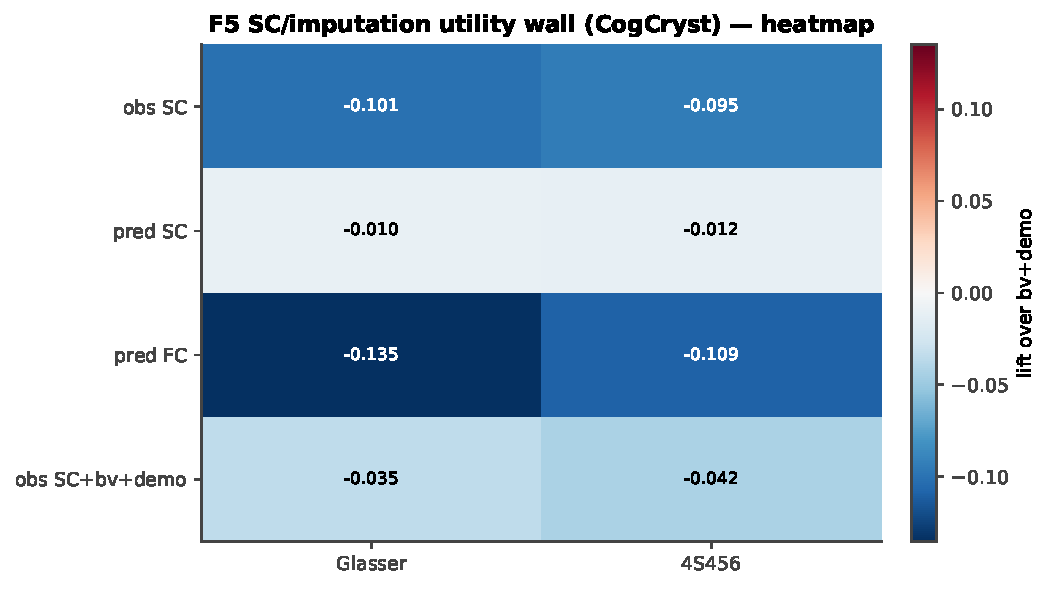
\includegraphics[height=0.82\textheight,width=\linewidth,keepaspectratio]{F5_v_heatmap.pdf}
\end{frame}
\begin{frame}{F5 · SC / imputation utility wall}{lollipop}
\centering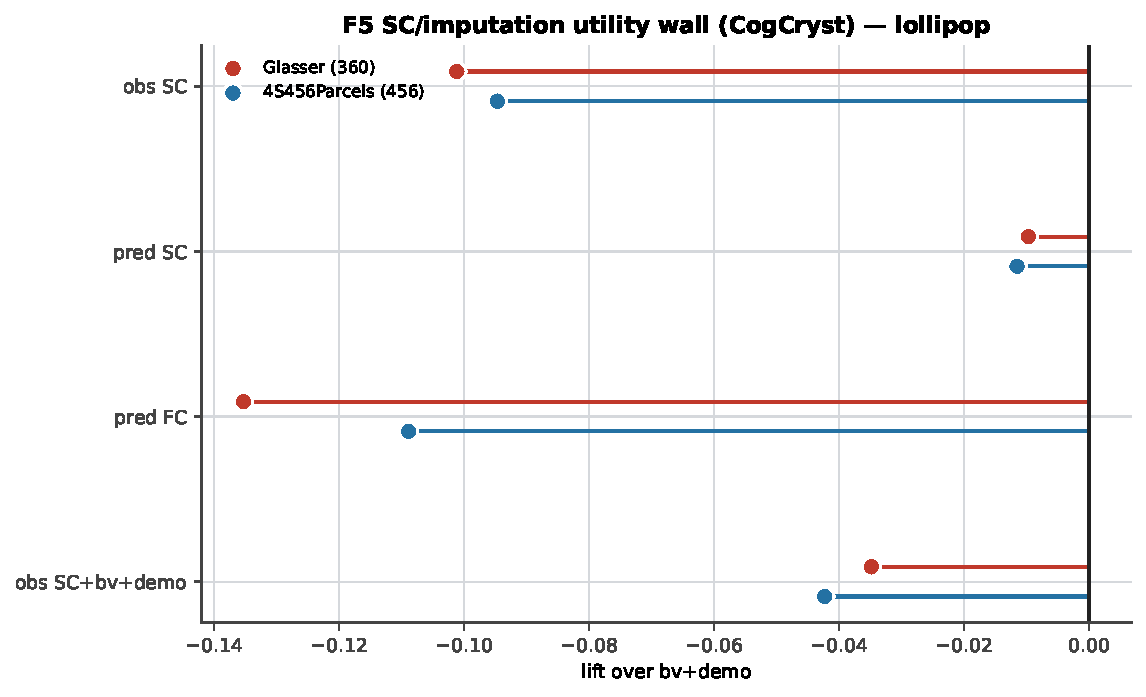
\includegraphics[height=0.82\textheight,width=\linewidth,keepaspectratio]{F5_v_lollipop.pdf}
\end{frame}
\begin{frame}{F5 · SC / imputation utility wall}{slope across parcellations}
\centering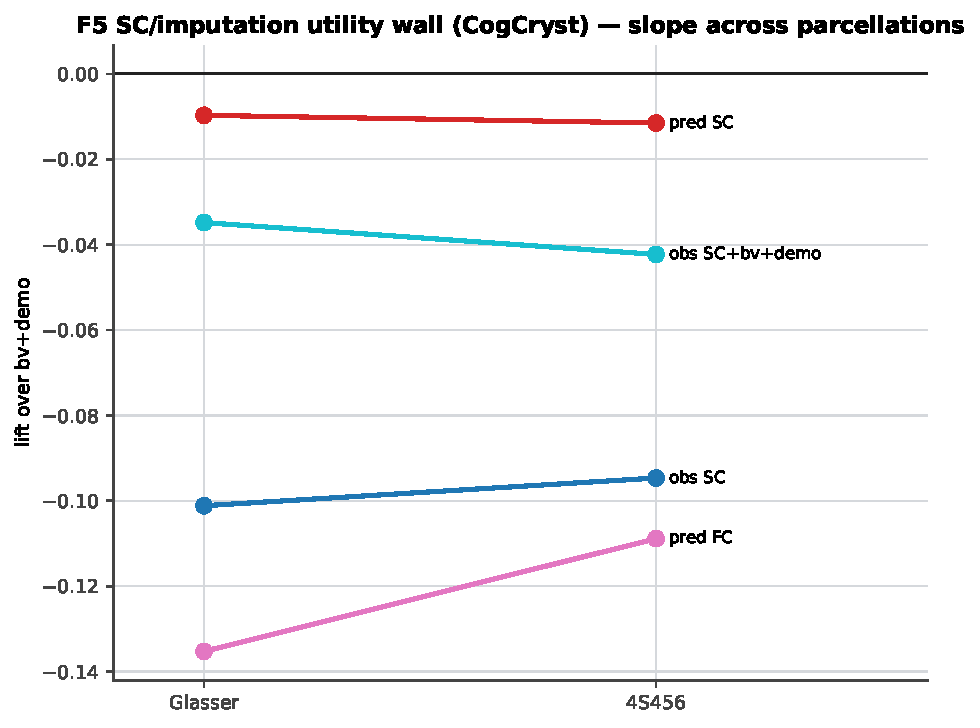
\includegraphics[height=0.82\textheight,width=\linewidth,keepaspectratio]{F5_v_slope.pdf}
\end{frame}
\section{F6}
\begin{frame}\centering\Large\textbf{F6 · Predicted connectomes carry family signal}\\[4pt]\normalsize 6 chart variants\end{frame}
\begin{frame}{F6 · Predicted connectomes carry family signal}{dumbbell (parcellation gap)}
\centering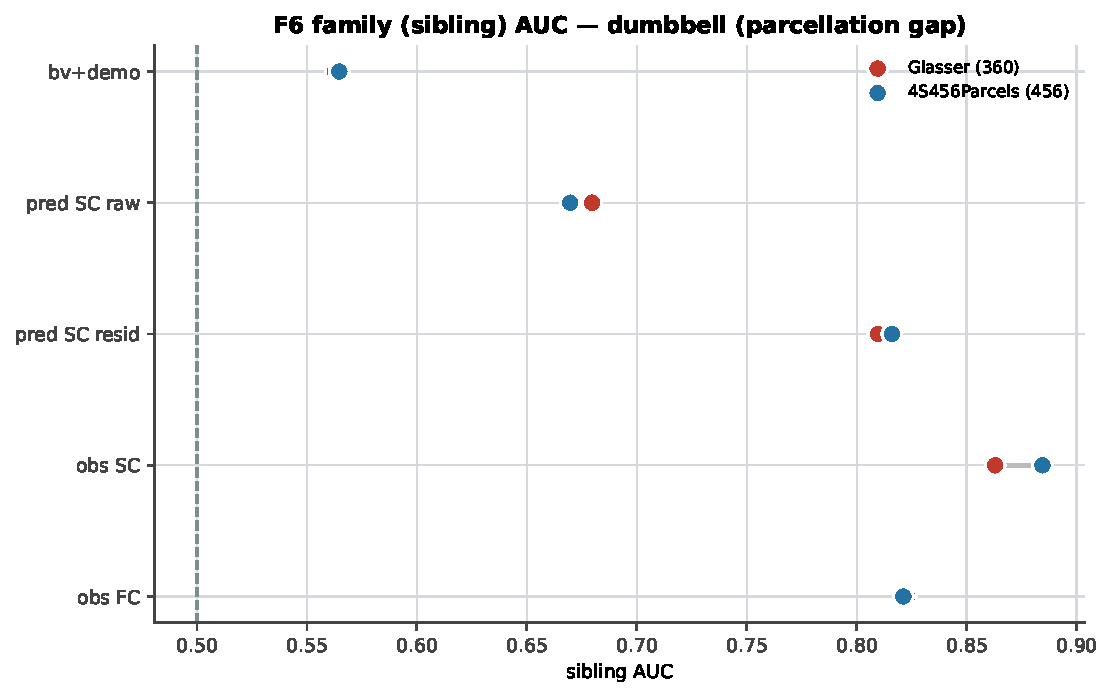
\includegraphics[height=0.82\textheight,width=\linewidth,keepaspectratio]{F6_v_dumbbell.pdf}
\end{frame}
\begin{frame}{F6 · Predicted connectomes carry family signal}{grouped bars}
\centering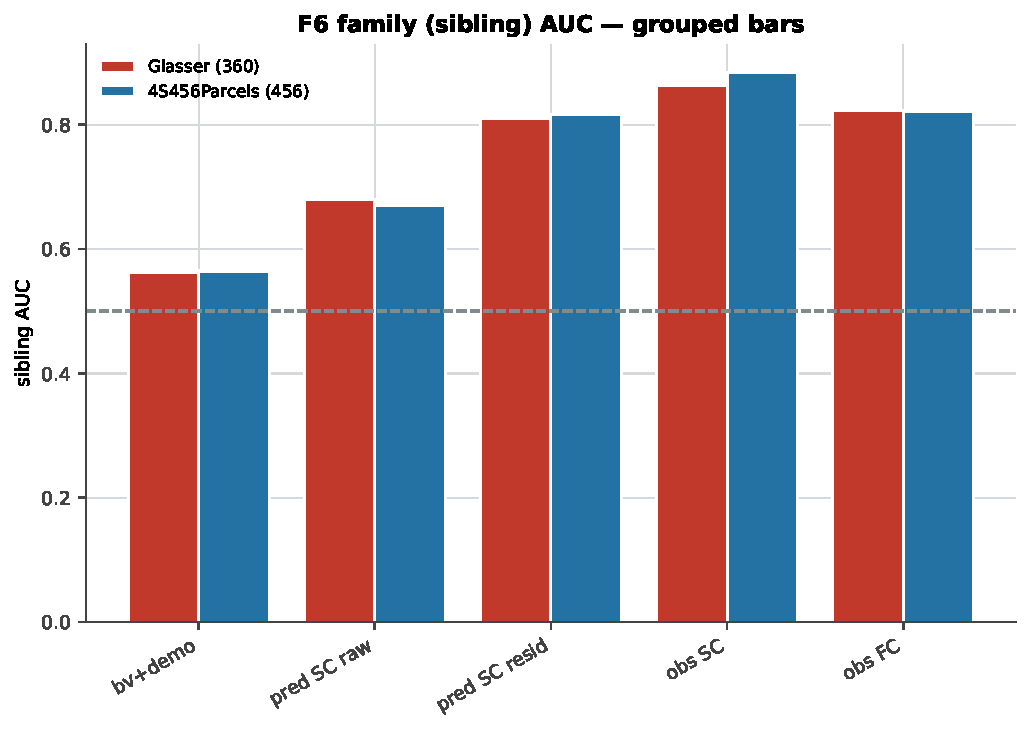
\includegraphics[height=0.82\textheight,width=\linewidth,keepaspectratio]{F6_v_groupedbar.pdf}
\end{frame}
\begin{frame}{F6 · Predicted connectomes carry family signal}{horizontal bars}
\centering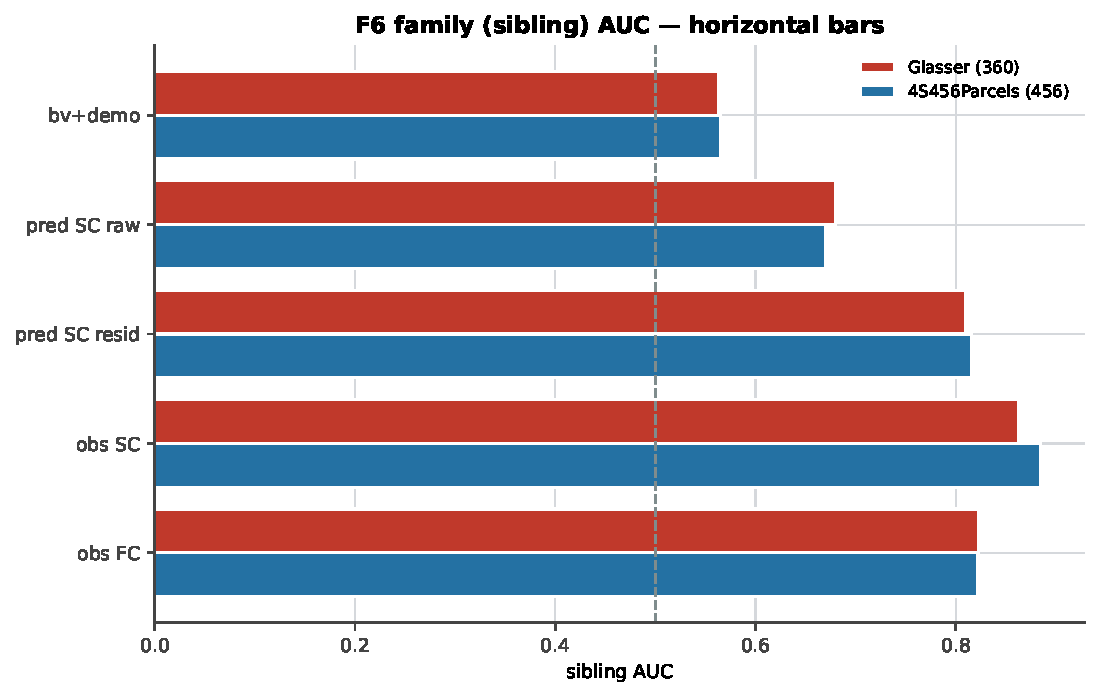
\includegraphics[height=0.82\textheight,width=\linewidth,keepaspectratio]{F6_v_hbar.pdf}
\end{frame}
\begin{frame}{F6 · Predicted connectomes carry family signal}{heatmap}
\centering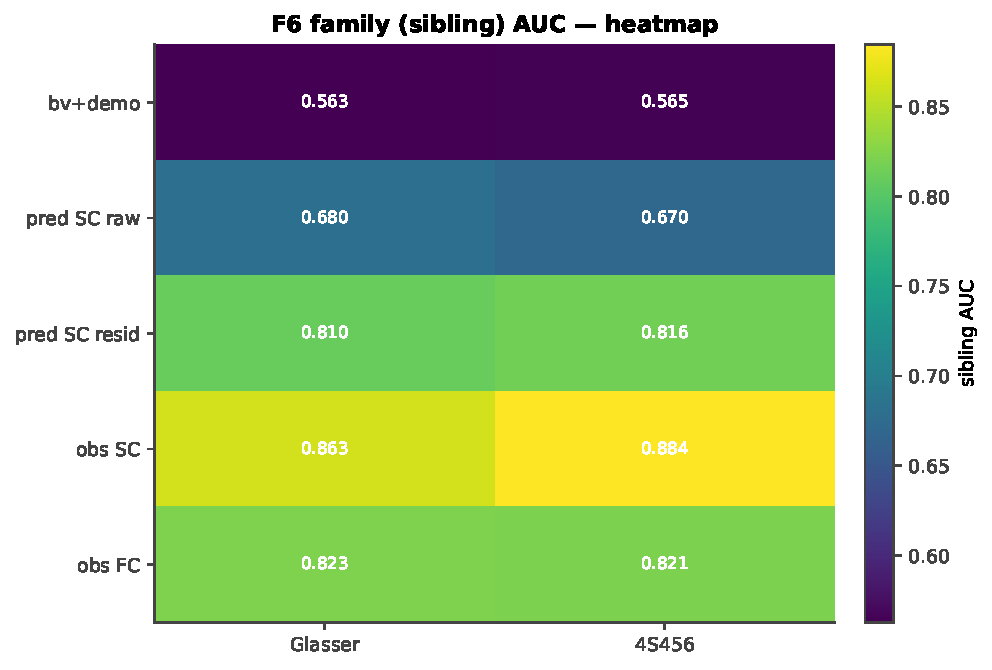
\includegraphics[height=0.82\textheight,width=\linewidth,keepaspectratio]{F6_v_heatmap.pdf}
\end{frame}
\begin{frame}{F6 · Predicted connectomes carry family signal}{lollipop}
\centering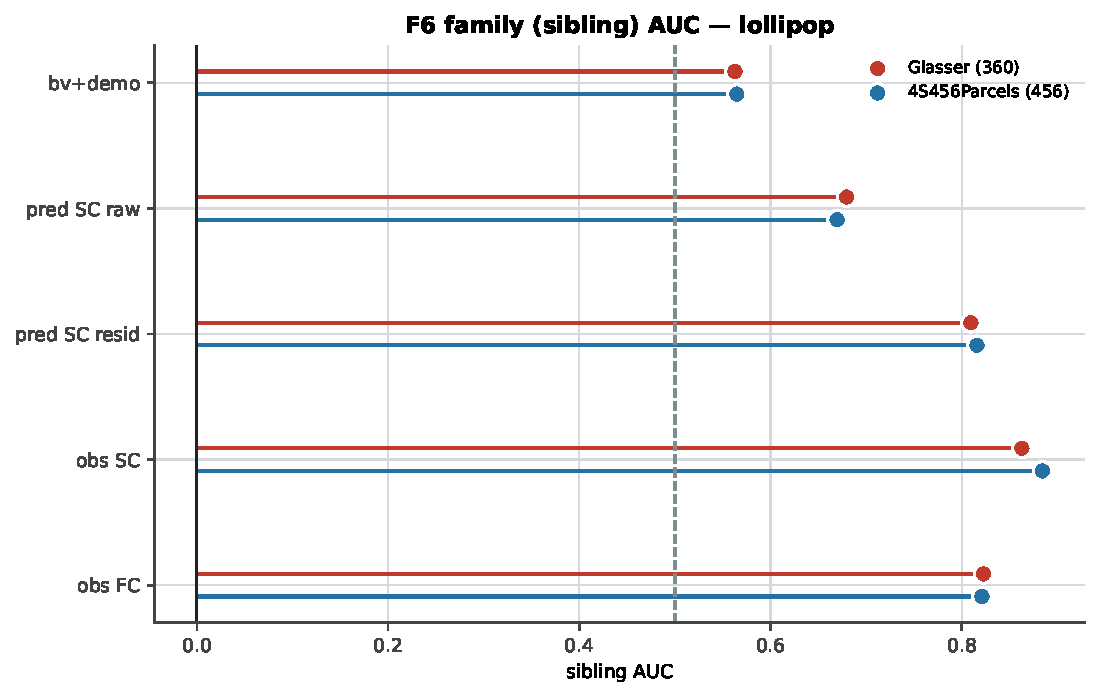
\includegraphics[height=0.82\textheight,width=\linewidth,keepaspectratio]{F6_v_lollipop.pdf}
\end{frame}
\begin{frame}{F6 · Predicted connectomes carry family signal}{slope across parcellations}
\centering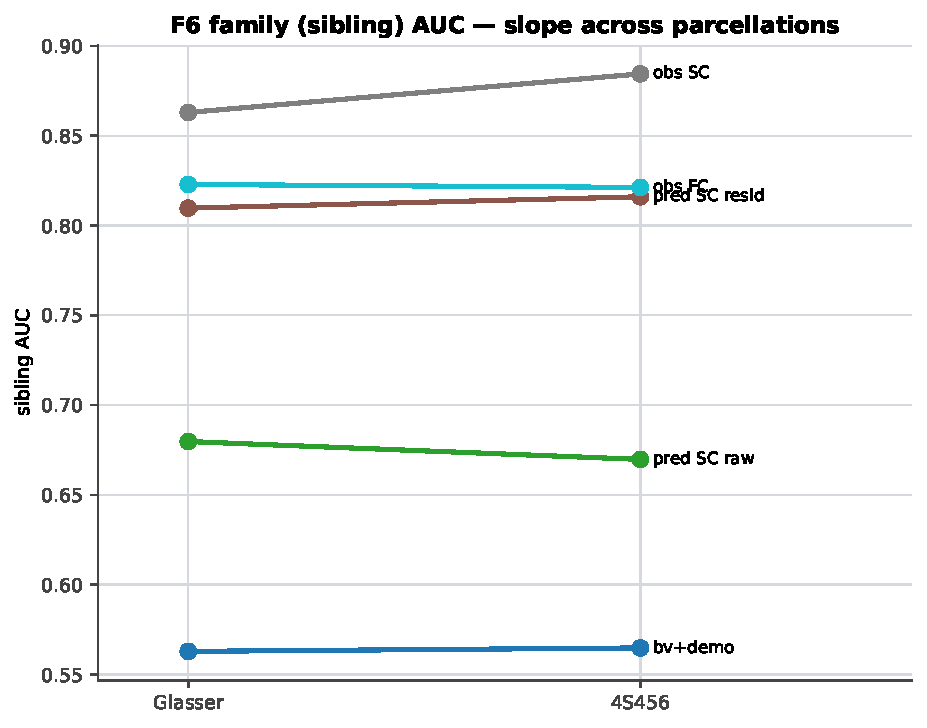
\includegraphics[height=0.82\textheight,width=\linewidth,keepaspectratio]{F6_v_slope.pdf}
\end{frame}
\section{F7}
\begin{frame}\centering\Large\textbf{F7 · Reconstruction vs identification tradeoff}\\[4pt]\normalsize 2 chart variants\end{frame}
\begin{frame}{F7 · Reconstruction vs identification tradeoff}{4S456Parcels}
\centering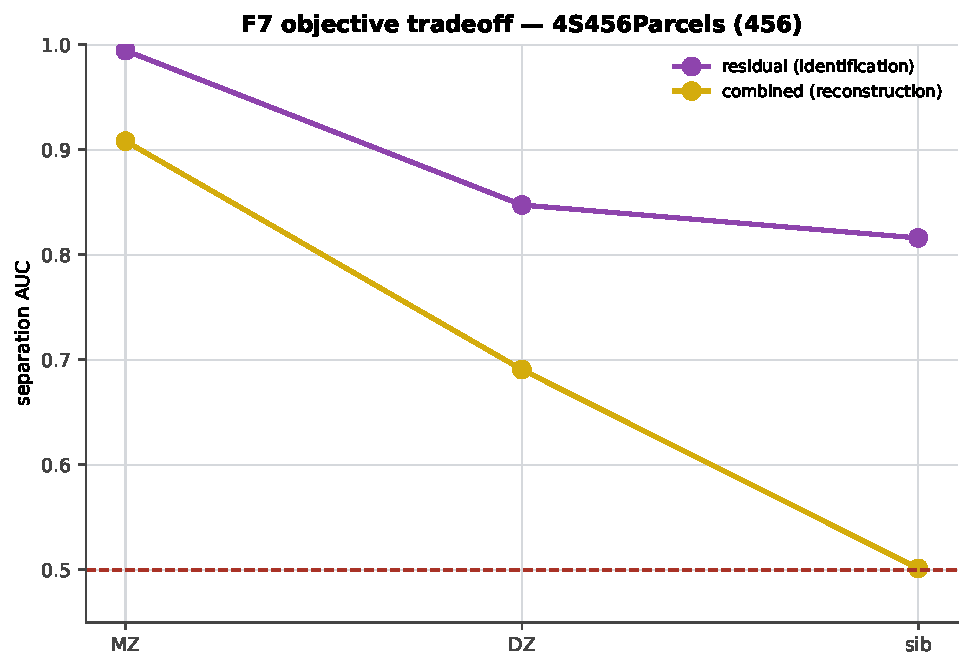
\includegraphics[height=0.82\textheight,width=\linewidth,keepaspectratio]{F7_v_4S456.pdf}
\end{frame}
\begin{frame}{F7 · Reconstruction vs identification tradeoff}{Glasser}
\centering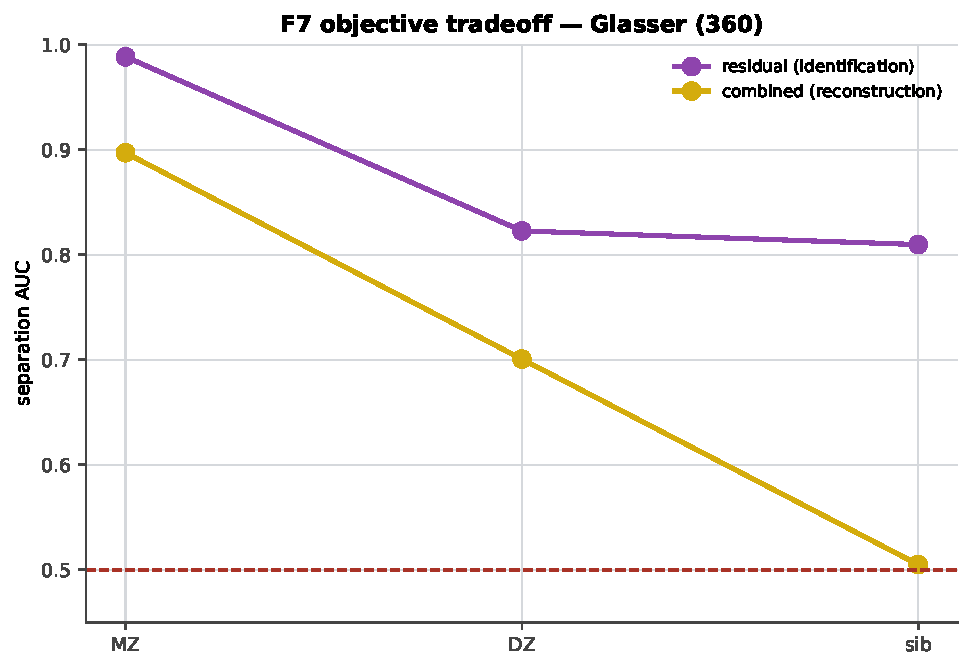
\includegraphics[height=0.82\textheight,width=\linewidth,keepaspectratio]{F7_v_Glasser.pdf}
\end{frame}
\section{F8}
\begin{frame}\centering\Large\textbf{F8 · FC-predictable low-variance SC mode (component index not stable)}\\[4pt]\normalsize 3 chart variants\end{frame}
\begin{frame}{F8 · FC-predictable low-variance SC mode (component index not stable)}{sibling AUC per PC}
\centering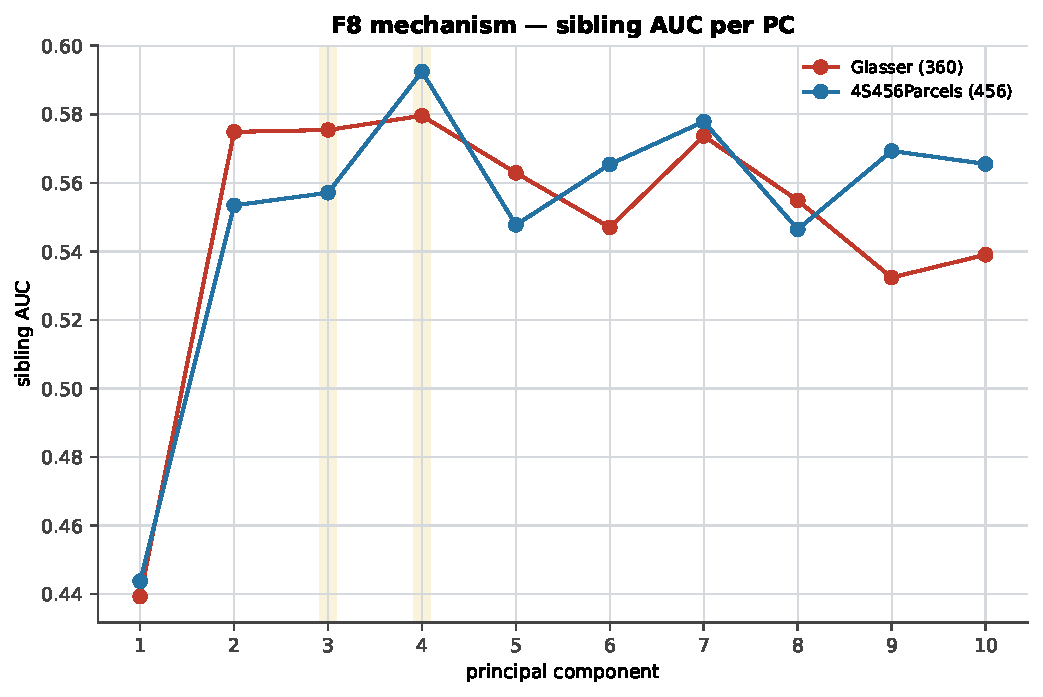
\includegraphics[height=0.82\textheight,width=\linewidth,keepaspectratio]{F8_v_auc.pdf}
\end{frame}
\begin{frame}{F8 · FC-predictable low-variance SC mode (component index not stable)}{sex/volume confound per PC}
\centering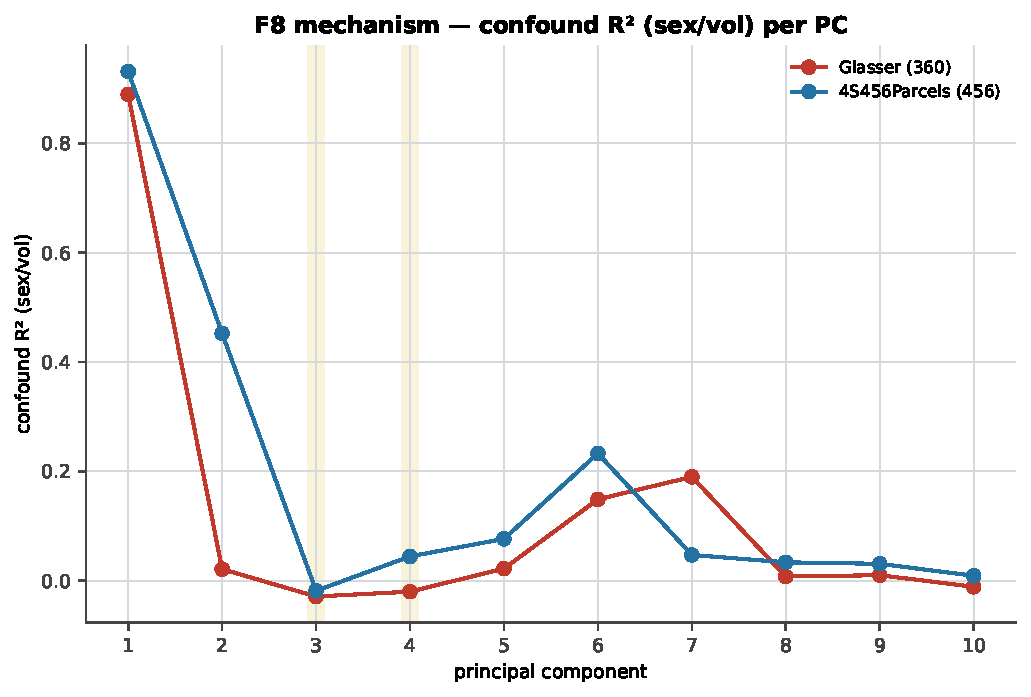
\includegraphics[height=0.82\textheight,width=\linewidth,keepaspectratio]{F8_v_conf.pdf}
\end{frame}
\begin{frame}{F8 · FC-predictable low-variance SC mode (component index not stable)}{FC→PC predictability per PC}
\centering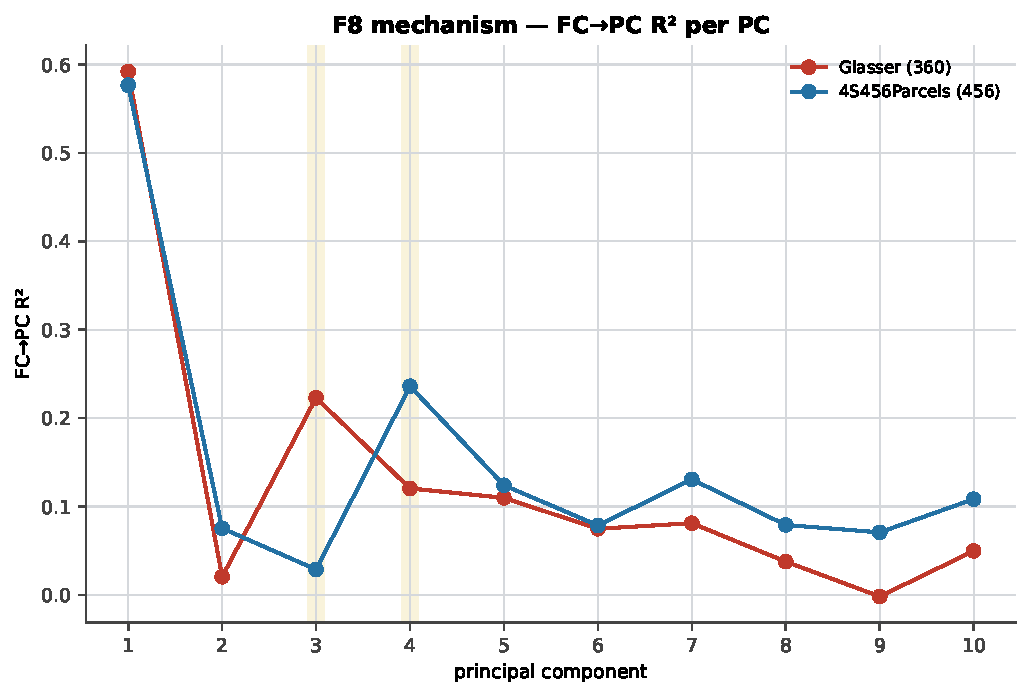
\includegraphics[height=0.82\textheight,width=\linewidth,keepaspectratio]{F8_v_fcr2.pdf}
\end{frame}
\section{F9}
\begin{frame}\centering\Large\textbf{F9 · Richer tractography does not help}\\[4pt]\normalsize 3 chart variants\end{frame}
\begin{frame}{F9 · Richer tractography does not help}{downstream cognition}
\centering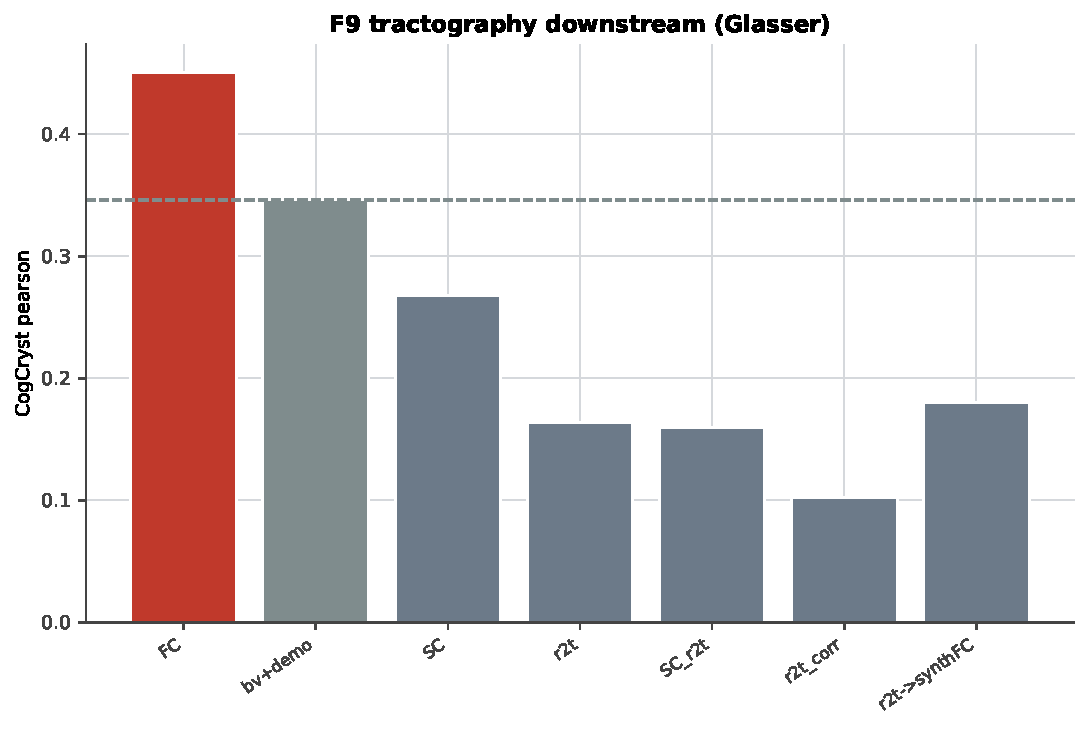
\includegraphics[height=0.82\textheight,width=\linewidth,keepaspectratio]{F9_v_downstream.pdf}
\end{frame}
\begin{frame}{F9 · Richer tractography does not help}{→FC bars}
\centering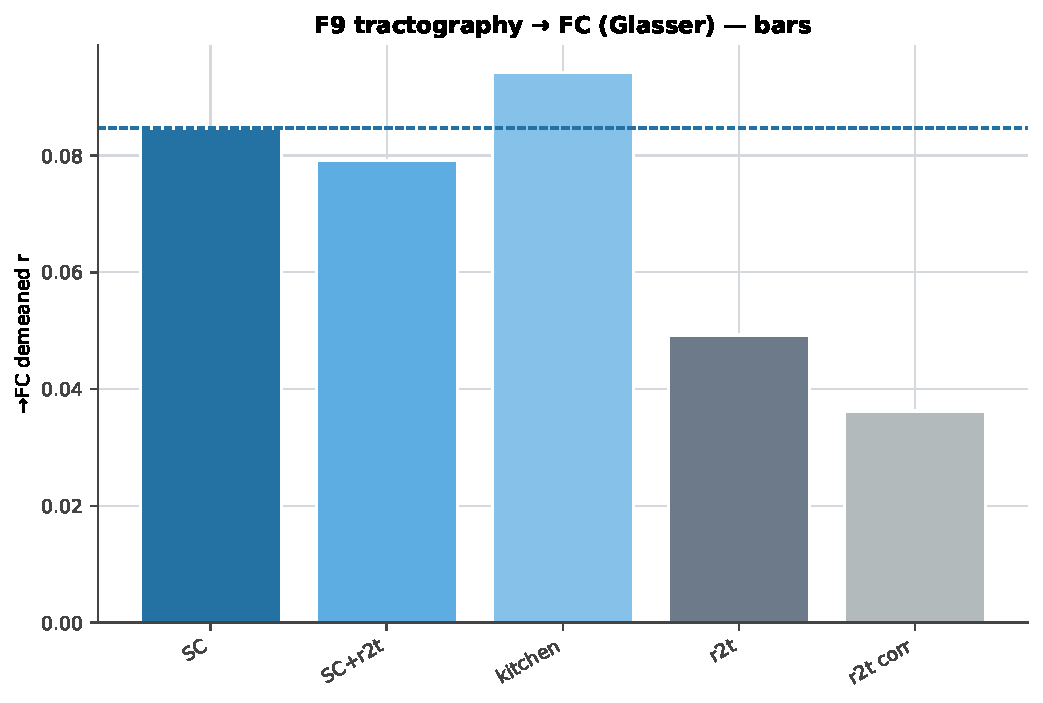
\includegraphics[height=0.82\textheight,width=\linewidth,keepaspectratio]{F9_v_recon_bar.pdf}
\end{frame}
\begin{frame}{F9 · Richer tractography does not help}{→FC hbar}
\centering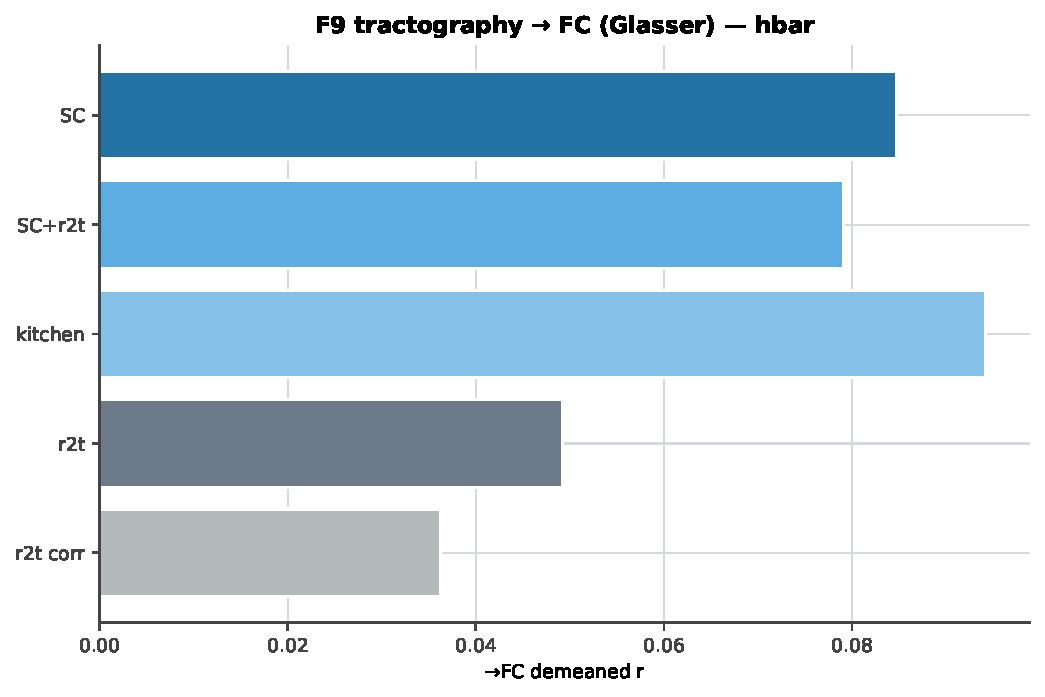
\includegraphics[height=0.82\textheight,width=\linewidth,keepaspectratio]{F9_v_recon_hbar.pdf}
\end{frame}
\section{F10}
\begin{frame}\centering\Large\textbf{F10 · The ceiling is structural}\\[4pt]\normalsize 3 chart variants\end{frame}
\begin{frame}{F10 · The ceiling is structural}{vs FC reliability ceiling}
\centering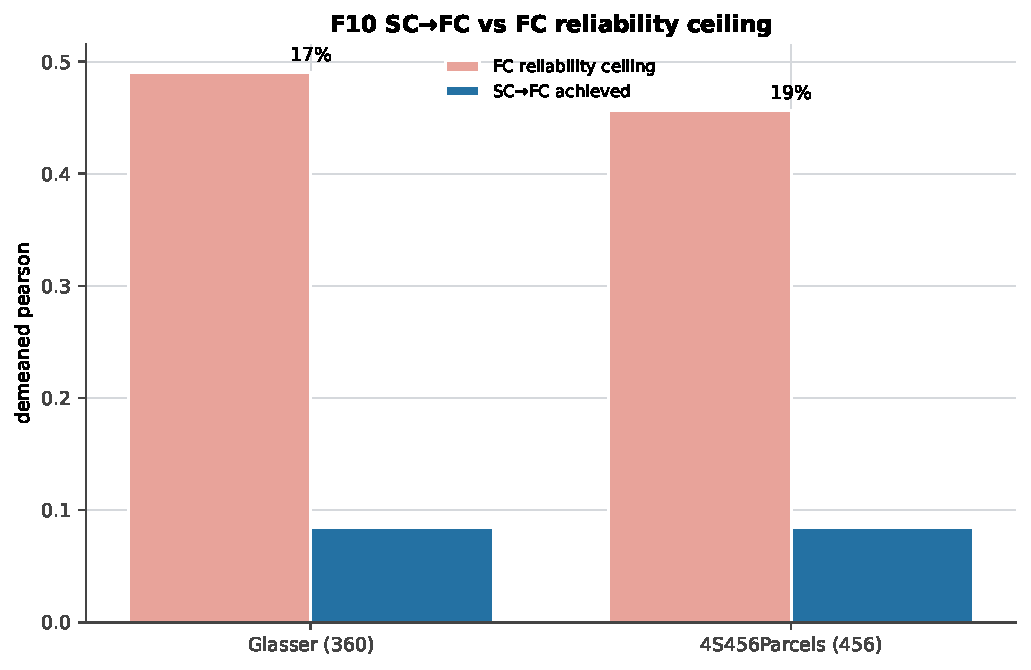
\includegraphics[height=0.82\textheight,width=\linewidth,keepaspectratio]{F10_v_ceiling.pdf}
\end{frame}
\begin{frame}{F10 · The ceiling is structural}{nonlinear gap vs n}
\centering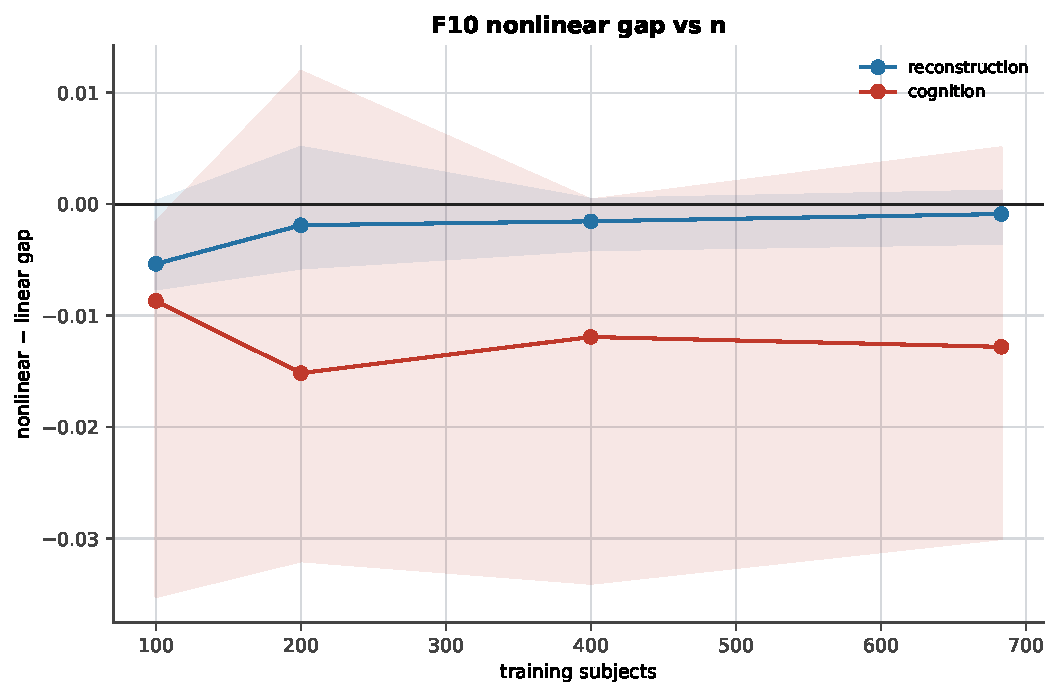
\includegraphics[height=0.82\textheight,width=\linewidth,keepaspectratio]{F10_v_gap.pdf}
\end{frame}
\begin{frame}{F10 · The ceiling is structural}{linear vs nonlinear vs n}
\centering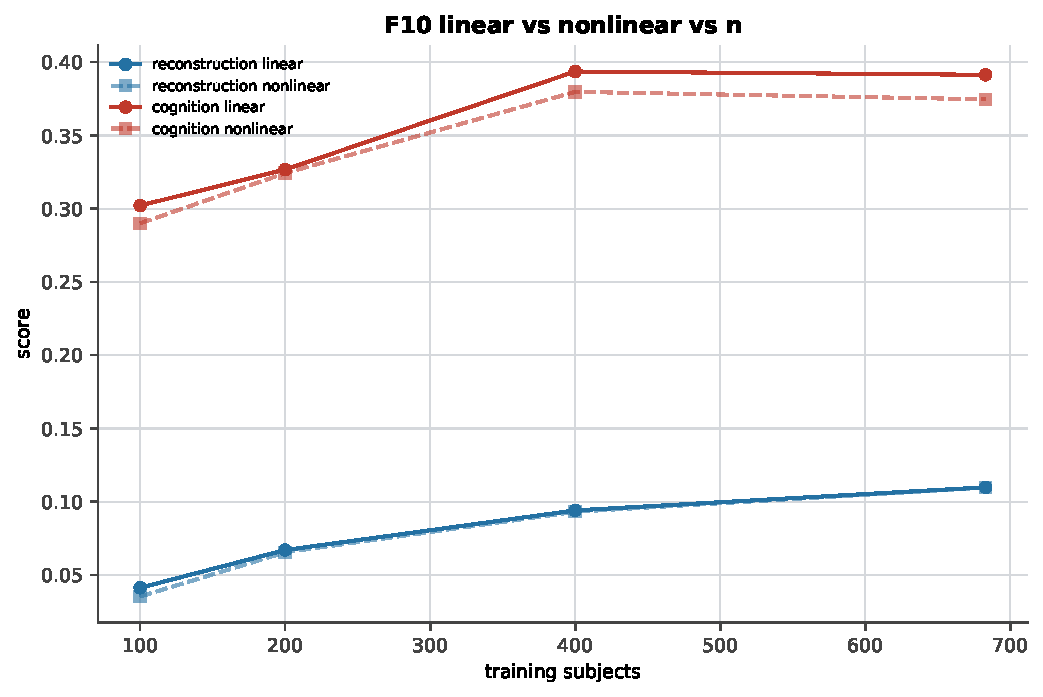
\includegraphics[height=0.82\textheight,width=\linewidth,keepaspectratio]{F10_v_linvsnon.pdf}
\end{frame}
\section{F11}
\begin{frame}\centering\Large\textbf{F11 · The cognition lift is multiplicity-fragile}\\[4pt]\normalsize 1 chart variants\end{frame}
\begin{frame}{F11 · The cognition lift is multiplicity-fragile}{full composite panel}
\centering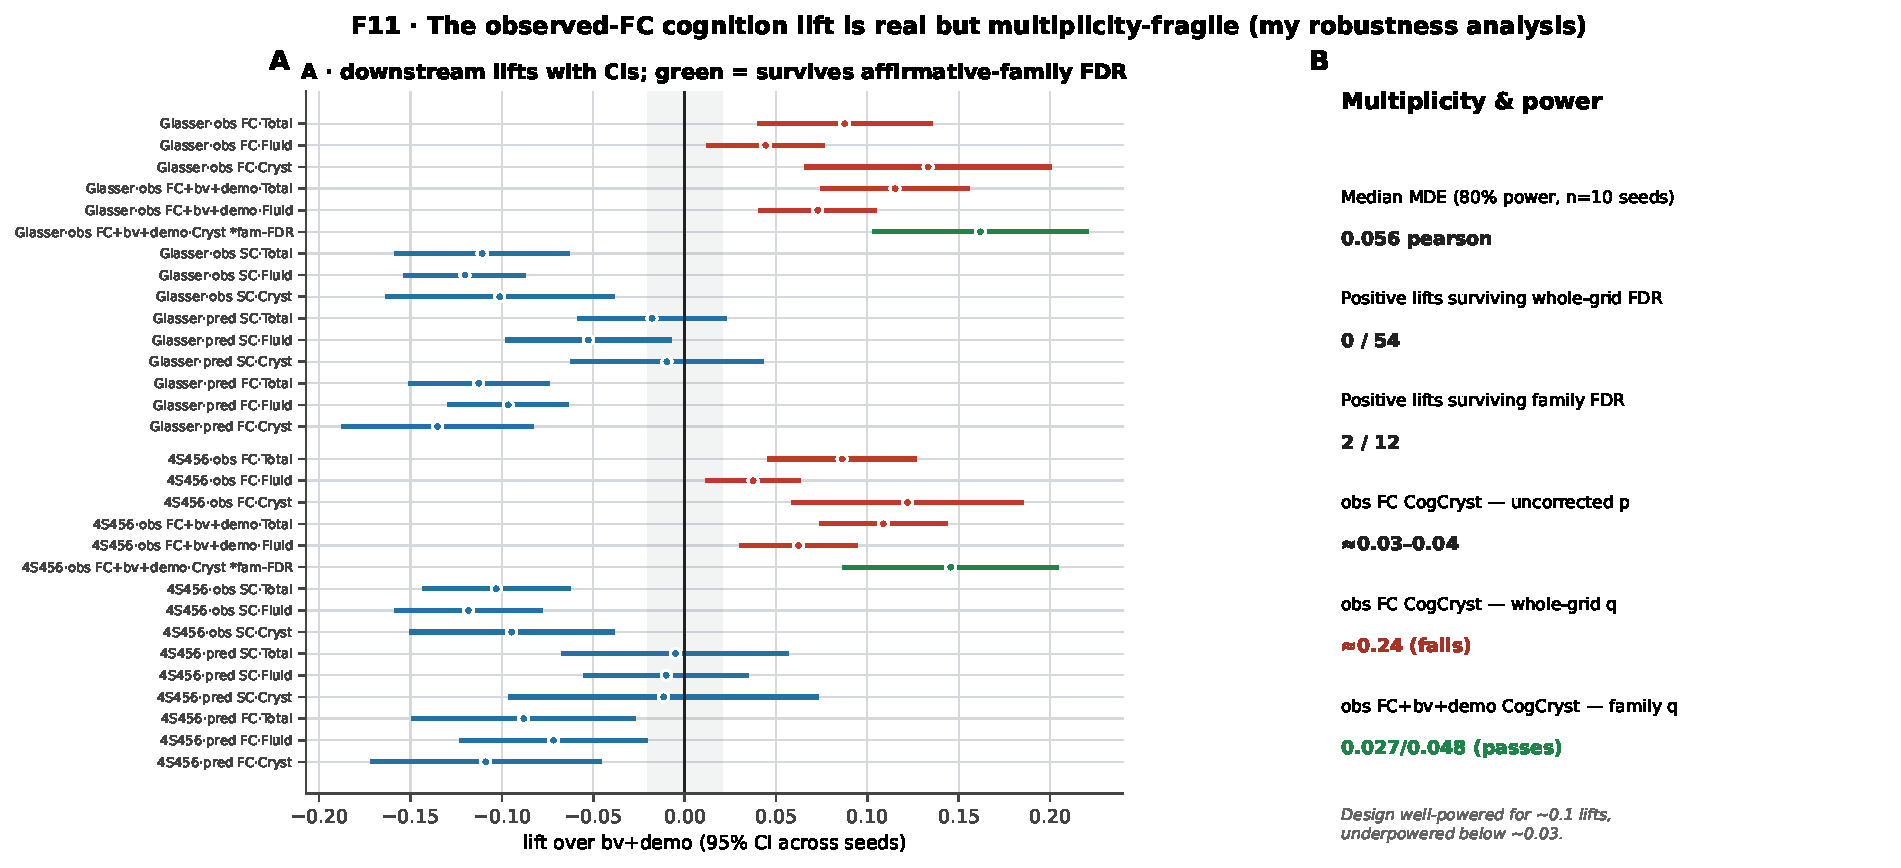
\includegraphics[height=0.82\textheight,width=\linewidth,keepaspectratio]{F11_v_composite.pdf}
\end{frame}
\section{F12}
\begin{frame}\centering\Large\textbf{F12 · Bayesian corroboration}\\[4pt]\normalsize 1 chart variants\end{frame}
\begin{frame}{F12 · Bayesian corroboration}{full composite panel}
\centering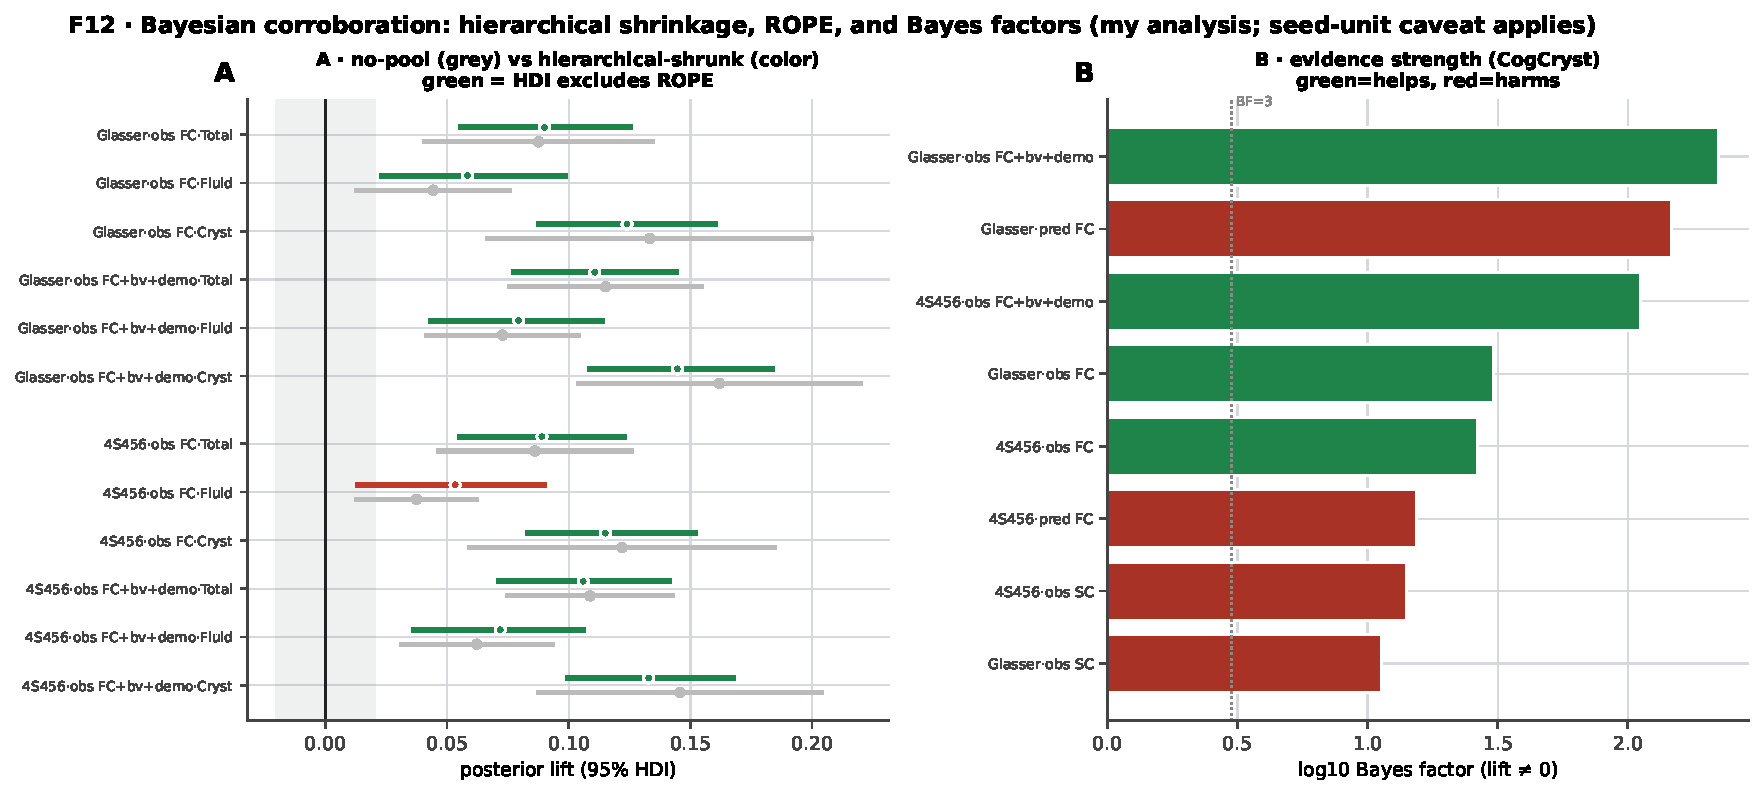
\includegraphics[height=0.82\textheight,width=\linewidth,keepaspectratio]{F12_v_composite.pdf}
\end{frame}
\section{F13}
\begin{frame}\centering\Large\textbf{F13 · Imputation harm / cross-modal loss}\\[4pt]\normalsize 7 chart variants\end{frame}
\begin{frame}{F13 · Imputation harm / cross-modal loss}{box + seed dots}
\centering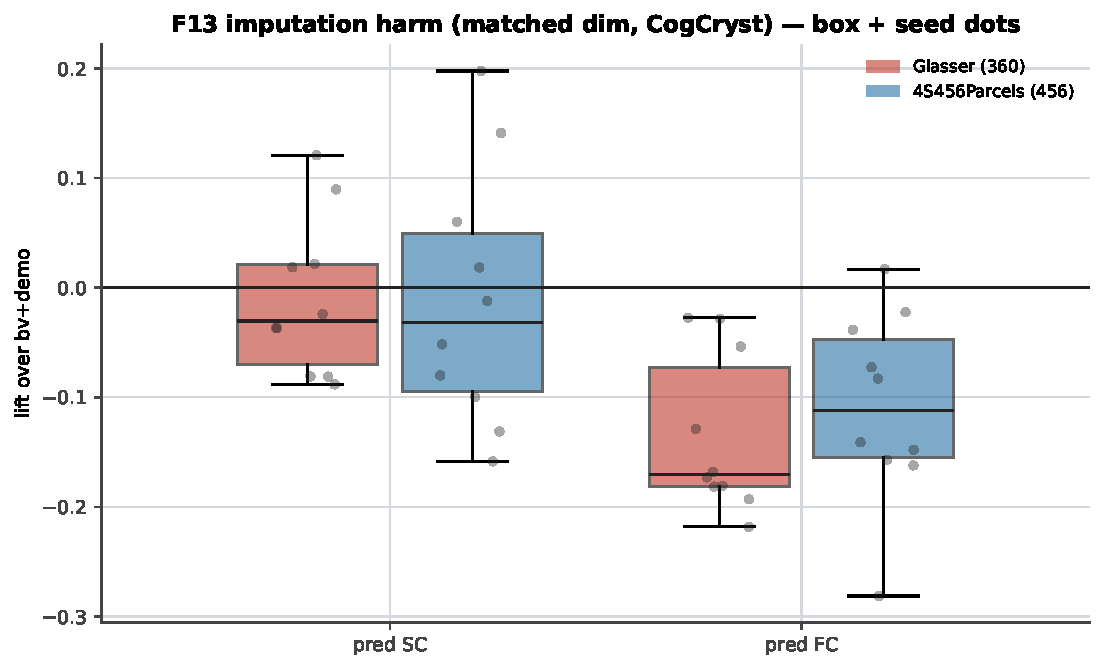
\includegraphics[height=0.82\textheight,width=\linewidth,keepaspectratio]{F13_v_box.pdf}
\end{frame}
\begin{frame}{F13 · Imputation harm / cross-modal loss}{dumbbell (parcellation gap)}
\centering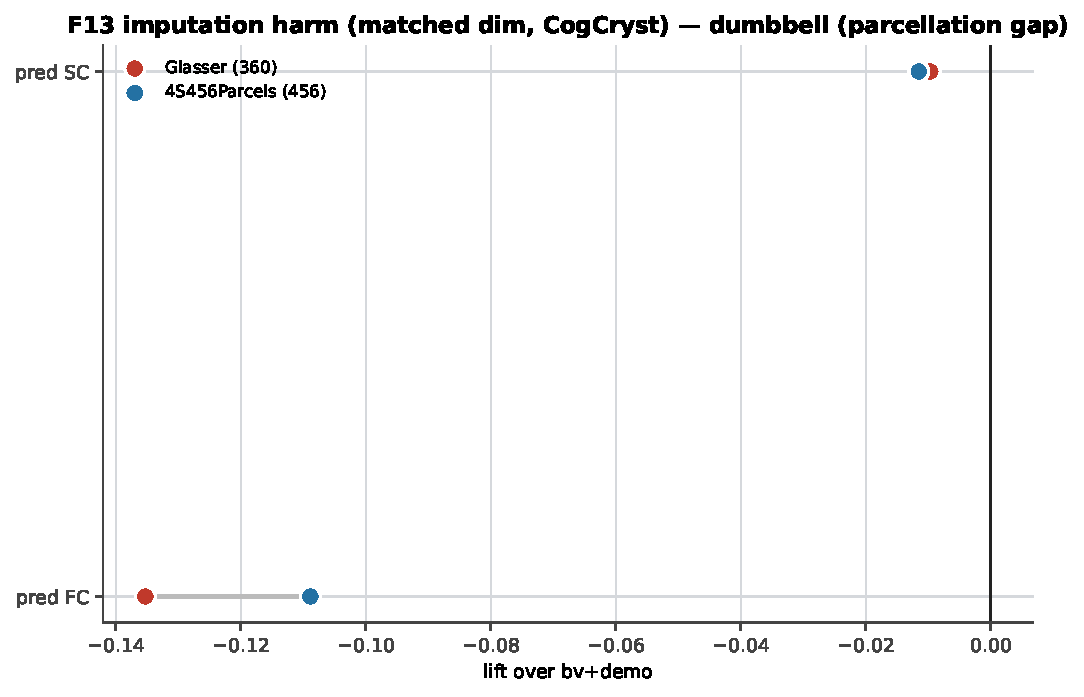
\includegraphics[height=0.82\textheight,width=\linewidth,keepaspectratio]{F13_v_dumbbell.pdf}
\end{frame}
\begin{frame}{F13 · Imputation harm / cross-modal loss}{grouped bars}
\centering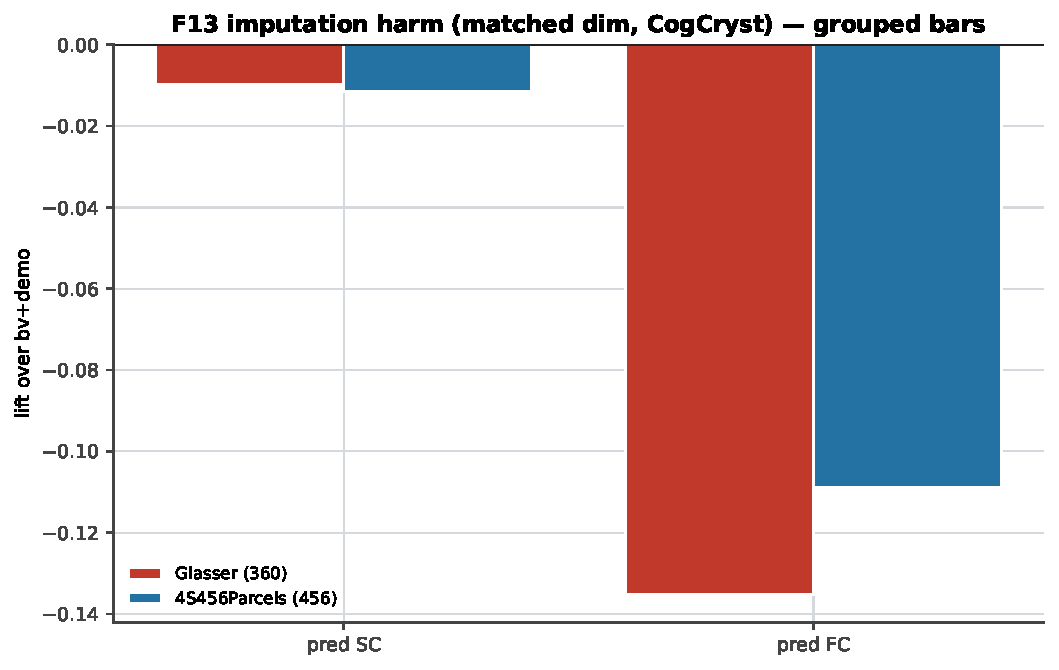
\includegraphics[height=0.82\textheight,width=\linewidth,keepaspectratio]{F13_v_groupedbar.pdf}
\end{frame}
\begin{frame}{F13 · Imputation harm / cross-modal loss}{horizontal bars}
\centering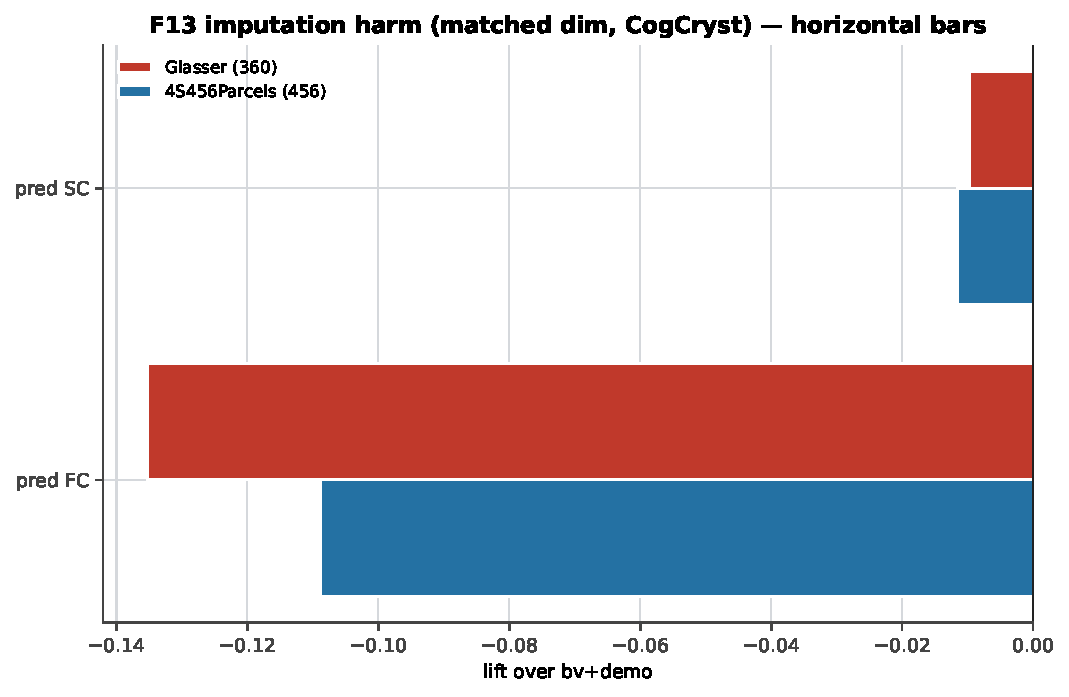
\includegraphics[height=0.82\textheight,width=\linewidth,keepaspectratio]{F13_v_hbar.pdf}
\end{frame}
\begin{frame}{F13 · Imputation harm / cross-modal loss}{heatmap}
\centering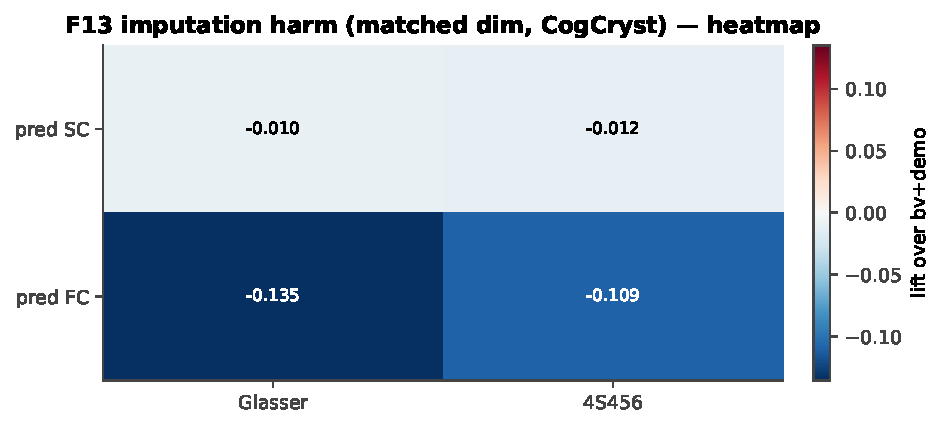
\includegraphics[height=0.82\textheight,width=\linewidth,keepaspectratio]{F13_v_heatmap.pdf}
\end{frame}
\begin{frame}{F13 · Imputation harm / cross-modal loss}{lollipop}
\centering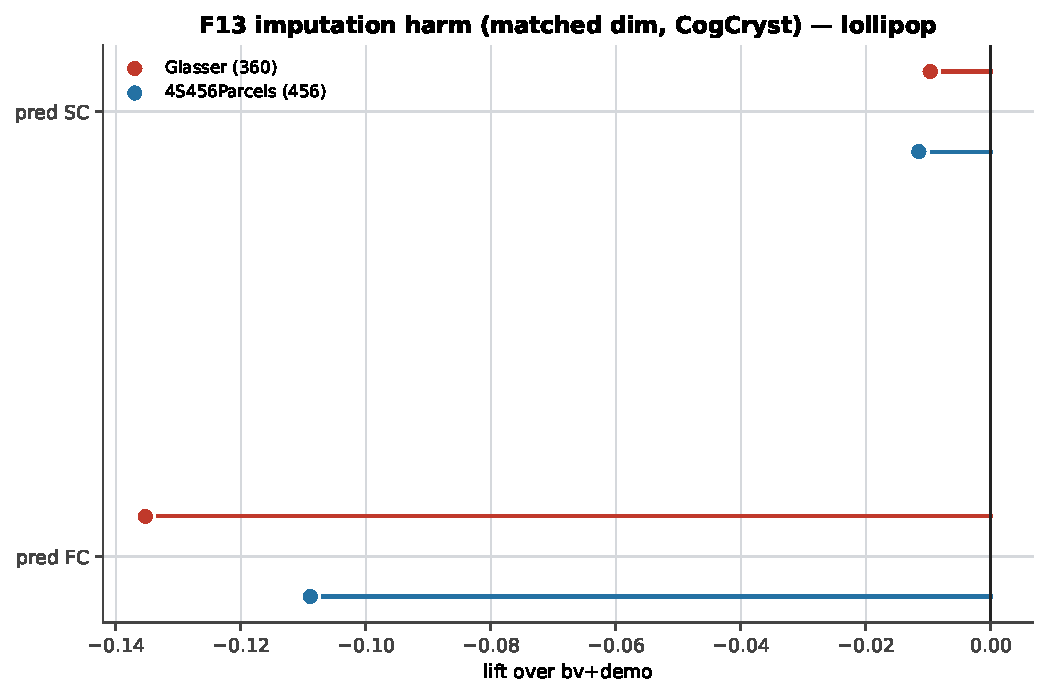
\includegraphics[height=0.82\textheight,width=\linewidth,keepaspectratio]{F13_v_lollipop.pdf}
\end{frame}
\begin{frame}{F13 · Imputation harm / cross-modal loss}{slope across parcellations}
\centering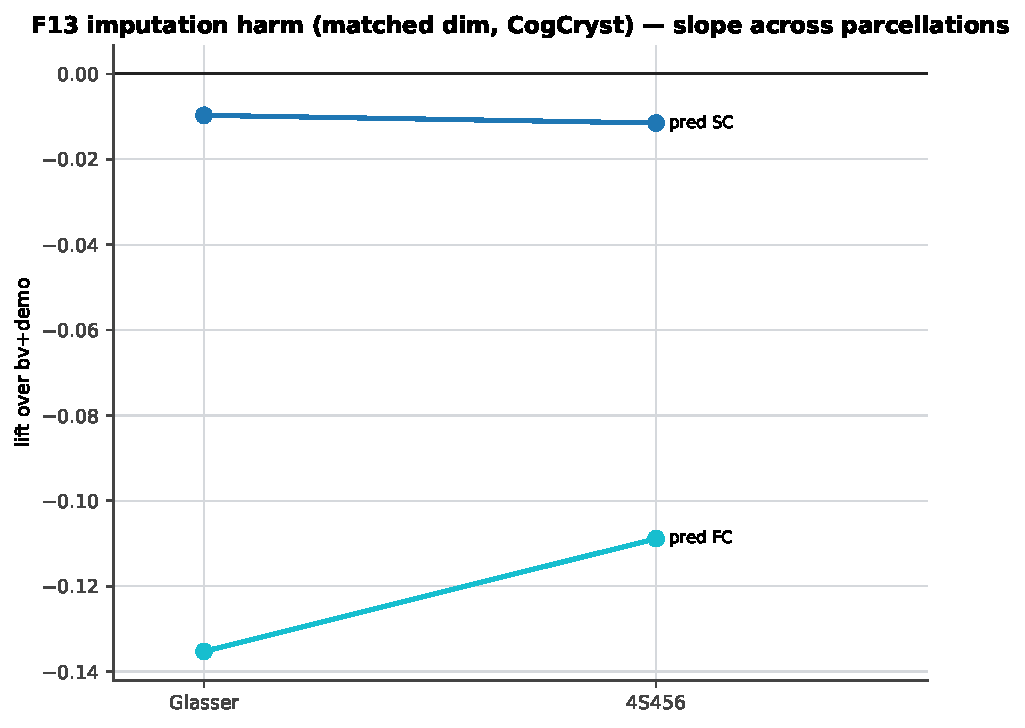
\includegraphics[height=0.82\textheight,width=\linewidth,keepaspectratio]{F13_v_slope.pdf}
\end{frame}
\end{document}